\documentclass[english,bachelor,uks]{webisthesis} % Weimar
% \documentclass[german,bachelor,fsu]{webisthesis} % Jena
% \documentclass[german,bachelor,ul]{webisthesis} % Leipzig
% \documentclass[german,master,buw,web]{webisthesis} % Weimar, for web page
% \documentclass[german,bachelor,fsu,web]{webisthesis} % Jena, for web page
% \documentclass[german,bachelor,ul,web]{webisthesis} % Leipzig, for web page
%
% Non-default programme
% ---------------------
% \documentclass[english,master,buw]{webisthesis}\global\thesisprogramme{Human-Computer Interaction}
% \documentclass[english,master,buw]{webisthesis}\global\thesisfrontpagefaculty{Faculty of Civil Engineering/Faculty of Media}\global\thesisprogramme{Digital Engineering}
% \documentclass[german,bachelor,buw]{webisthesis}\global\thesisprogramme{Informatik\\Schwerpunkt Medieninformatik}
% \documentclass[german,bachelor,buw]{webisthesis}\global\thesisprogramme{Informatik\\Schwerpunkt Security and Data Science}
%
% When you change the language, pdflatex may halt on recompilation.
% Just hit enter to continue and recompile again. This should fix it.


%
% Values
% ------
\ThesisSetTitle{Learning Heuristics for Efficient Causal Question Answering Using A* Search}
\ThesisSetKeywords{Causal Question Answering, Causal Knowledge Graphs, A* Search, Heuristic Graph Search, Sentence Embeddings, Matryoshka Embeddings, Graph Traversal}
\ThesisSetLocation{Kassel}

\ThesisSetAuthor{Ashkan Kiafard}
\ThesisSetStudentNumber{35825953}
\ThesisSetDateOfBirth{23}{06}{2002}
\ThesisSetPlaceOfBirth{Iran}

% Supervisors should usually be Professors from the candidate's university. A second supervisor is not always needed.
\ThesisSetSupervisors{Prof.\ Dr.\ Martin Potthast,Prof.\ Dr.\ Oliver Hohlfeld}

\ThesisSetSubmissionDate{9}{9}{2026}

%
% Suggested Packages
% ------------------
\usepackage[numbers,sort&compress]{natbib}
%   Allows citing in different ways (e.g., only the authors if you use the
%   citation again within a short time).
%
\usepackage{booktabs}
%    For tables ``looking the right way''.
%
% \usepackage{tabularx}
%    Enables tables with columns that automatically fill the page width.
%
% \usepackage[ruled,algochapter]{algorithm2e}
%    A package for pseudo code algorithms.
%
\usepackage{amsmath}
%    For tabular-style formatting of mathematical environments.
%

\usepackage{fontawesome}
%    For lots of awesome glyphs: https://mirror.physik.tu-berlin.de/pub/CTAN/fonts/fontawesome/doc/fontawesome.pdf

\usepackage{amssymb}
\usepackage{graphicx}

%
% Commenting (by your supervisor)
% -------------------------------
\usepackage{xcolor}
\usepackage{soul}
\newcommand{\bscom}[2]{%
  % #1 Original text.
  % #2 Replacement text.
    \st{\scriptsize\,#1}{\color{blue}\scriptsize\,#2}%
  }

\usepackage{float}
\usepackage{array}
\usepackage{algorithm}
\usepackage[bottom]{footmisc}
\usepackage{algpseudocode}
\usepackage{siunitx}
\sisetup{
    group-separator = {,},
    group-minimum-digits = 4
}

% Create links in the pdf document
% Hyperref has some incompatibilities with other packages
% Some other packages must be loaded before, some after hyperref
% Additional options to the hyperref package can be provided in the braces [], like in
% \usehyperref[backref] % This will add back references in the bibliography that some people like ... some don't ... so better ask your supervisor ;-)
\usehyperref

\begin{document}
\begin{frontmatter}


\begin{abstract}
Many information needs are causal, asking why events occur, what consequences they have, or whether one event leads to another. Such questions arise across domains including healthcare, economics, public policy, and environmental science. A fundamental task is answering the binary question \mbox{``Does $A$ cause $B$?''} While large language models can answer such questions directly, their responses may hallucinate causal relationships and often lack an explicit causal path. Causal graphs instead encode causal knowledge explicitly by representing concepts or events as nodes and causal relationships as directed edges. This allows binary causal question answering to be formulated as directed pathfinding, where an answer can be supported by an explicit path from $A$ to $B$. Exhaustive pathfinding methods such as Breadth-First Search (BFS) become expensive on large causal graphs. This thesis proposes an embedding-guided $A^*$ method for efficient causal path discovery. Embedding distances are used as edge costs and heuristic estimates toward the target concept. Off-the-shelf sentence embeddings already provide useful search guidance, while fine-tuning further reduces search effort. Matryoshka Representation Learning enables compact embeddings and allows the trade-off between search efficiency and effectiveness to be controlled through embedding dimensionality. Experiments on binary causal question answering datasets derived from \mbox{MS MARCO} and SemEval across CauseNet Precision, \mbox{CauseNet Full}, and CEG Filtered show efficiency gains. On the larger \mbox{CauseNet Full} and \mbox{CEG Filtered} graphs, the selected $A^*$ configuration is at least $1.3\times$ as fast as capped BFS and $8.2\times$ as fast as uncapped BFS, while reducing the number of visited nodes by factors of at least $5.9$ and $107$, respectively. Compared with the reinforcement learning approach of \citeauthor{bluebaum:2024}, it achieves higher F\textsubscript{1} in all final test settings while being at least $56\times$ as fast. Overall, the results show that learning an embedding-based heuristic provides an efficient alternative to exhaustive and neural graph traversal.
\end{abstract}



\tableofcontents

% \chapter*{Acknowledgements} % optional
% I thank the authors of the webisthesis template for their excellent work!

% \listoffigures % optional, usually not needed

% \listoftables % optional, usually not needed

% \listofalgorithms % optional, usually not needed
%    requires package algorithm2e

% optional: list of symbols/notation (e.g., using the nomencl package) but usually not needed
\end{frontmatter}

\chapter{Introduction}

Many questions about real-world phenomena are causal in nature, from medical diagnosis~\cite{richens:2020} to analyzing the effects of policies~\cite{blackwell:2013} or environmental changes~\cite{guevara:2025}. Humans can approach such questions using domain knowledge, experience, and intuition. Answering them automatically, however, requires causal knowledge in a machine-processable form. While causal information can be extracted from large text collections, its unstructured nature makes algorithmic reasoning difficult. Causal graphs provide a structured representation using nodes for concepts or events and directed edges for causal relationships, enabling causal reasoning via graph traversal. The binary question of whether a concept $A$ causes another concept~$B$ can therefore be formulated as a pathfinding problem from $A$ to $B$. Causal graphs such as CauseNet~\cite{heindorf:2020} contain millions of cause--effect relationships extracted from the web, making efficient traversal a challenge.\looseness=-1

A straightforward approach is exhaustive search using Breadth-First Search (BFS), which guarantees completeness and shortest paths in terms of hop count~\cite{cormen:2022}. However, shortest paths are not necessarily the most semantically meaningful. Due to the noisy, automatically extracted nature of large causal graphs, they may include weak or overly general causal links, limiting their usefulness as explanations. For example, in CauseNet, BFS connects \textit{waves} to \textit{destruction} through the path \textit{waves} $\rightarrow$ \textit{death} $\rightarrow$ \textit{destruction}. Although topologically valid, the highly connected intermediate concept \textit{death} provides only a broad connection between the queried concepts. In addition, BFS becomes computationally expensive in graphs with high branching factors, often requiring the exploration of thousands of nodes before reaching the target. To reduce this search space, a reinforcement learning (RL) traversal approach has been proposed~\cite{bluebaum:2024}. This approach learns a policy to guide exploration toward promising regions of the graph, substantially reducing the number of visited nodes. However, maintaining and evaluating a dedicated neural policy introduces architectural complexity and inference overhead.

To make causal question answering more efficient, this thesis replaces the learned traversal policy with a learned search heuristic, removing neural computations from graph traversal at inference time. The proposed approach employs $A^*$ search with the embedding distance between the current and target nodes as its heuristic. A pretrained sentence transformer provides embeddings that guide the search toward semantically closer nodes, reducing unnecessary exploration. Since semantic proximity alone does not necessarily identify the most promising successor, the embeddings are further fine-tuned for the search objective. Training examples are derived from $A^*$ paths that reach the target, teaching the model to favor successors that provide a shorter embedding-space route toward the target. In the previous example, $A^*$ with the fine-tuned embeddings instead finds the equally short path \mbox{\textit{waves} $\rightarrow$ \textit{turbulence} $\rightarrow$ \textit{destruction}}, replacing the broad intermediate concept \textit{death} with the more specific \textit{turbulence}. Empirical evaluation shows that fine-tuning substantially reduces the number of visited nodes while generally retaining competitive effectiveness. BFS remains more effective in some settings, but its search effort increases substantially on larger graphs. Compared with the RL method of Blübaum and Heindorf~\cite{bluebaum:2024}, the proposed approach achieves F\textsubscript{1} scores at least \(7.3\) percentage points higher across all final test settings while being at least \(56\times\) as fast.

The contributions of this thesis are as follows: (1) an embedding-guided \(A^*\) approach is proposed for efficient binary causal question answering over large-scale causal graphs; (2) a search-oriented fine-tuning procedure adapts the embedding space for causal pathfinding, together with Matryoshka Representation Learning to support efficient low-dimensional heuristics; and (3) a systematic evaluation on in-domain and out-of-domain causal graphs and datasets compares the approach with BFS and RL traversal, demonstrating substantial reductions in search effort and runtime while characterizing the resulting effectiveness--efficiency trade-off.

The remainder of this thesis is structured as follows:
The theoretical foundations required for the proposed approach are introduced in Chapter~\ref{chap:foundations}. Related work on causal question answering, causal graphs, and graph traversal methods, including RL-based approaches and learned search heuristics, is reviewed in Chapter~\ref{chap:related_work}. Chapter~\ref{chap:methodology} then presents the problem formulation and the proposed embedding-guided \(A^*\) approach for causal graph traversal. The training procedure, including supervision construction, fine-tuning, validation, and model selection, is described in Chapter~\ref{chap:train}. Experimental evaluation and comparisons with BFS and RL across different datasets and causal graphs follow in Chapter~\ref{chap:results}. Chapter~\ref{chap:discussion} discusses the main findings, trade-offs, and limitations. Finally, Chapter~\ref{chap:conclusion} summarizes the thesis and outlines future work.


\chapter{Foundations}
\label{chap:foundations}

This chapter introduces the theoretical concepts required for the remainder of this thesis. Section~\ref{sec:foundations_graphs} formalizes causal graphs and defines binary causal questions as reachability problems. Section~\ref{sec:foundations_astar} presents heuristic search and the $A^*$ algorithm. Section~\ref{sec:foundations_repr} introduces transformer-based embedding models and their use for graph search. Section~\ref{sec:foundations_matryoshka} presents Matryoshka Representation Learning. Finally, Section~\ref{sec:foundations_activation} introduces the non-linear activation functions used within the training objective.

\section{Causal Graphs and Binary Causal Questions}
\label{sec:foundations_graphs}

Causal knowledge graphs provide a structured representation of causal relationships that would otherwise remain implicit in unstructured text~\cite{heindorf:2020,li:2020}. They can be modeled as directed graphs \(G=(V,E)\), where nodes represent concepts or events and directed edges encode causal relations between them. This structure enables algorithmic reasoning over causal dependencies. Figure~\ref{fig:causal_types} illustrates three common causal structures, namely a causal chain, a common cause, and a common effect. Given two concepts $A$ and $B$, let $a,b \in V$ denote their corresponding graph nodes. The binary question ``Does $A$ cause $B$?'' then reduces to determining whether a directed path exists from $a$ to $b$~\cite{bluebaum:2024}\looseness=-1:
\[
\exists \; (a = v_0, v_1, \dots, v_k = b)
\text{ such that }
\forall i \in \{0,\dots,k-1\} \; (v_i, v_{i+1}) \in E.
\]
If such a path exists, the query is answered positively under this graph-based formulation. If no path can be found, either no causal relation is encoded in the graph or the available knowledge is incomplete. This formulation enables the application of classical graph traversal algorithms for causal reasoning.

\begin{figure}[t]
    \centering
    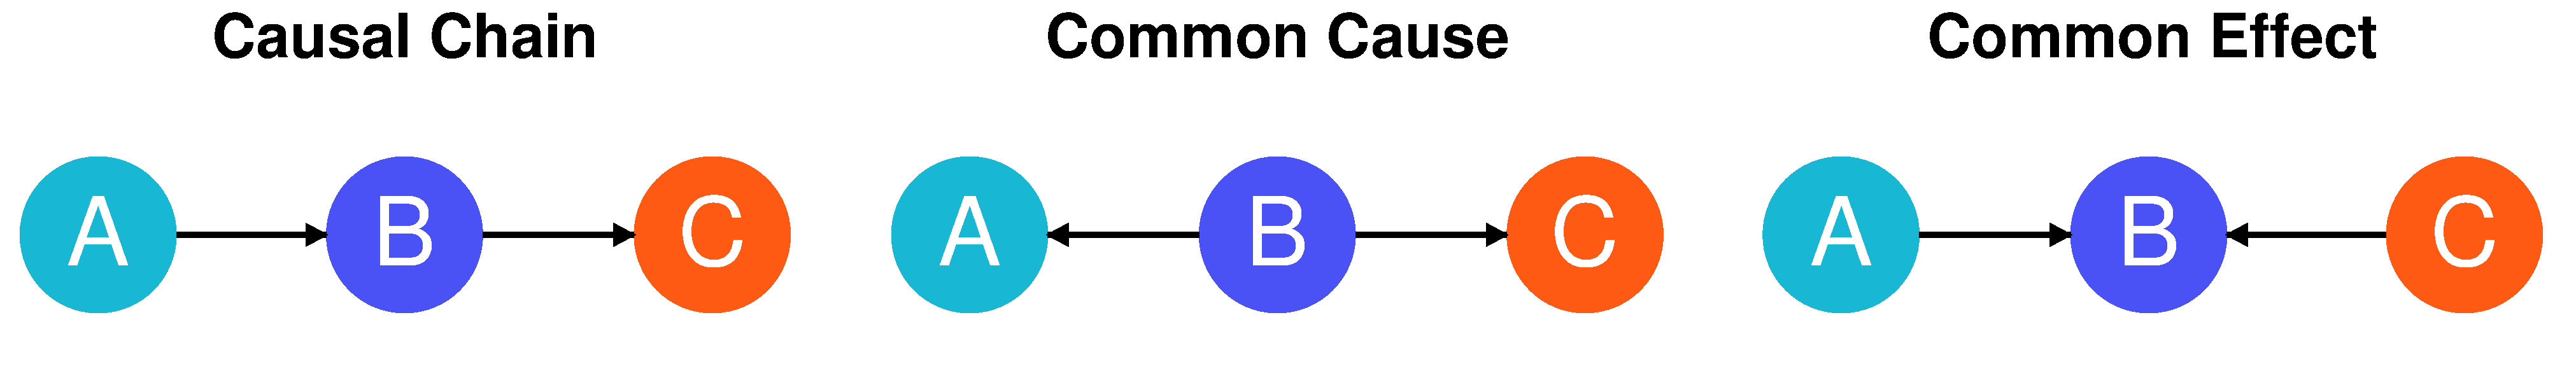
\includegraphics[width=\linewidth]{figures/causal_relation_patterns.pdf}
    \caption{Three common causal structures in directed graphs, showing a causal chain, a common cause, and a common effect.}
    \label{fig:causal_types}
\end{figure}

\section{Heuristic Search and the \texorpdfstring{$A^*$}{A*} Algorithm}
\label{sec:foundations_astar}

Graph traversal can be performed using uninformed or informed search algorithms. Uninformed search methods, such as BFS, explore the graph without guidance and guarantee completeness~\cite{cormen:2022}. However, their computational cost can be high in large graphs with significant branching factors. Heuristic search algorithms incorporate problem-specific information to guide exploration. The $A^*$ algorithm is an informed best-first search strategy~\cite{hart:1968} that selects nodes based on an evaluation function
\[
f(n) = g(n) + h(n),
\]
where $g(n)$ denotes the cost of the path from the start node to node $n$, $h(n)$ is a heuristic estimate of the remaining cost from $n$ to the target node, and $f(n)$ represents the estimated total cost of a solution path passing through $n$. At each step, $A^*$ expands the node with the smallest $f(n)$ value. The properties of $A^*$ depend on the quality of the heuristic function. Two important properties are consistency and admissibility~\cite{hart:1968}. A heuristic is \emph{consistent} if, for every node $n$ and each successor $s$, it satisfies
\[
h(n) \leq c(n,s) + h(s),
\]
where $c(n,s)$ is the cost of transitioning from $n$ to $s$. Consistency implies that $f$-values are non-decreasing along every path. Consequently, once a node has been expanded, it does not need to be reopened. A weaker condition is \emph{admissibility}, which requires that the heuristic never overestimates the true remaining cost:
\[
h(n) \leq d(n),
\]
where $d(n)$ denotes the optimal cost from node $n$ to the goal. If the heuristic is admissible, $A^*$ is guaranteed to find an optimal path when closed nodes can be reopened after a cheaper path is discovered. Without consistency, such re-expansions may be necessary.

\section{Representation Learning for Graph Search}
\label{sec:foundations_repr}

Modern natural language processing systems commonly represent textual concepts as dense vector embeddings. Transformer-based architectures form the basis of many state-of-the-art embedding models. A transformer encoder maps an input text sequence to contextualized token representations through self-attention mechanisms~\cite{vaswani:2017}. Sentence transformer models aggregate contextualized token representations into fixed-dimensional embeddings, forming a geometric space in which semantically related concepts tend to be located closer together~\cite{reimers:2019}. In graph search settings, such geometric structure can be used to guide exploration toward promising regions of the graph. Given two embeddings $\mathbf{x}, \mathbf{y} \in \mathbb{R}^d$, similarity or distance can be measured using metrics such as cosine similarity or Euclidean distance. Cosine similarity~\cite{manning:2008} is defined as
\[
\text{cosine}(\mathbf{x}, \mathbf{y}) =
\frac{\mathbf{x} \cdot \mathbf{y}}{\|\mathbf{x}\|\|\mathbf{y}\|}.
\]
It lies in the interval $[-1,1]$. In this work, cosine distance is computed as
\[
d_{\text{cos}}(\mathbf{x}, \mathbf{y}) = 1 - \text{cosine}(\mathbf{x}, \mathbf{y}),
\]
which lies in $[0,2]$. If either vector has zero norm, the cosine distance is set to $1.0$ to avoid division by zero. The second distance measure considered in this work is Euclidean distance~\cite{manning:2008}, defined as
\[
d_{\text{Euc}}(\mathbf{x}, \mathbf{y}) =
\|\mathbf{x} - \mathbf{y}\|_2.
\]
In this thesis, an embedding-guided variant of $A^*$ search is employed. Let $\phi(v)$ denote the embedding of node $v$. The cost of traversing an edge from node $n$ to a successor $s$ is defined as the distance between their embeddings, while $g(n)$ is the sum of these edge costs along the path from the start node to $n$. The heuristic $h(n)$ is the embedding distance from $n$ to the target node $b$. When Euclidean distance is used, consistency follows directly from the triangle inequality. For every successor $s$ of node $n$,
\[
h(n)
=
\lVert \phi(n)-\phi(b)\rVert_2
\leq
\lVert \phi(n)-\phi(s)\rVert_2
+
\lVert \phi(s)-\phi(b)\rVert_2
=
c(n,s)+h(s).
\]
The heuristic therefore satisfies the consistency condition of $A^*$. In contrast, cosine distance does not generally satisfy the standard triangle inequality and therefore does not guarantee heuristic consistency~\cite{schubert:2021}.

\section{Matryoshka Representation Learning}
\label{sec:foundations_matryoshka}

Standard embedding models are typically trained to produce representations with a fixed dimensionality. If such an embedding is truncated to a smaller number of dimensions, there is generally no guarantee that the reduced vector retains meaningful structure.
Matryoshka Representation Learning~\cite{kusupati:2022} addresses this limitation by optimizing multiple prefix subspaces of an embedding to remain informative. Let $\mathbf{e} \in \mathbb{R}^d$ denote a learned embedding vector with full dimensionality $d$. Instead of optimizing only the full representation, the model is trained such that several nested prefix dimensionalities
\[
m_1 < m_2 < \dots < m_k = d
\]
preserve useful structural information. For each dimensionality $m_i$, the corresponding truncated embedding is defined as
\[
\mathbf{e}_{m_i} = \mathbf{e}_{1:m_i},
\]
where $\mathbf{e}_{1:m_i}$ denotes the prefix consisting of the first $m_i$ components of the full embedding vector. The training objective is applied at multiple prefix dimensionalities, encouraging each truncated embedding to retain task-relevant information. This promotes an ordered representation in which earlier dimensions capture broadly useful features, while later dimensions add finer-grained information and additional capacity~\cite{kusupati:2022}. This property enables a trade-off between representational capacity and computational efficiency. In applications such as graph search, reducing embedding dimensionality can lower the cost of distance computations while preserving sufficient information for effective heuristic guidance. However, overly small prefixes may discard too much information and degrade the quality of the heuristic.

\section{Activation Functions}
\label{sec:foundations_activation}

Neural networks rely on non-linear activation functions to model complex relationships between inputs and outputs. Without non-linearities, stacked linear transformations would collapse into a single linear mapping, severely limiting representational power. One widely used activation function is the Rectified Linear Unit (ReLU)~\cite{nair:2010}, defined as
\[
\text{ReLU}(x) = \max(0, x).
\]
ReLU maps negative inputs to zero while preserving positive inputs. Its simple piecewise-linear form allows for efficient computation. Another commonly used activation function is the Gaussian Error Linear Unit (GELU)~\cite{hendrycks:2016}, defined as
\[
\text{GELU}(x) = x \cdot \Phi(x),
\]
where $\Phi(x)$ denotes the cumulative distribution function of the standard normal distribution.
\begin{figure}[htbp]
    \centering
    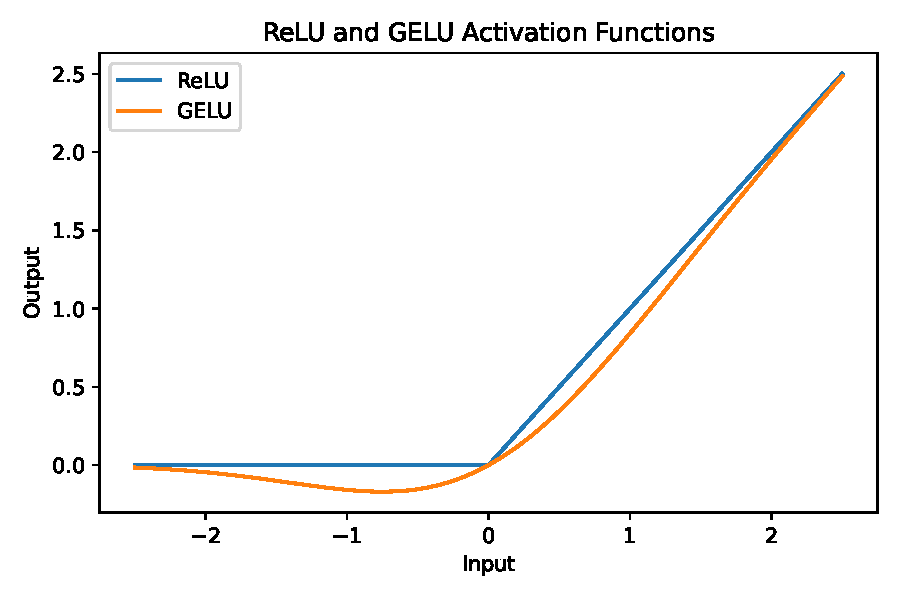
\includegraphics[width=1\linewidth]{figures/relu_gelu}
    \caption{Comparison of ReLU and GELU activation functions.}
    \label{fig:relu_gelu}
\end{figure}
In practical implementations, GELU is often approximated using a tanh-based formulation~\cite{hendrycks:2016}:
\[
\text{GELU}(x) \approx 0.5x \left(1 + \tanh\left(\sqrt{\frac{2}{\pi}} \left(x + 0.044715x^3\right)\right)\right),
\]
which provides a computationally efficient approximation while preserving the smooth gating behavior of the original function. Unlike ReLU, which applies a hard threshold at zero, GELU provides a smooth activation that weights inputs according to their magnitude. Figure~\ref{fig:relu_gelu} illustrates this difference. In this thesis, ReLU and GELU are evaluated as non-linear transformations within the training objective. Their different shapes determine how score differences are transformed and how strongly they contribute to the loss, thereby shaping the learned embedding space used by the $A^*$ heuristic.

\chapter{Related Work}
\label{chap:related_work}

This chapter reviews the main prior work on which this thesis builds. Section~\ref{sec:rw_causal_qa} introduces causal question answering and distinguishes between text-based and graph-based approaches. Section~\ref{sec:rw_causal_graphs} discusses causal knowledge graphs, their
construction, and their properties. Subsections~\ref{sec:rw_causenet} and~\ref{sec:rw_causalbank} present CauseNet and the Cause Effect Graph (CEG), the causal graph resources used in this work. Section 3.3 discusses the current state of the art in causal graph traversal, a reinforcement learning (RL) approach that addresses the same binary causal question answering task and therefore provides the most relevant point of comparison for this thesis. Finally, Section~\ref{sec:rw_learned_heuristics} reviews prior work on learned heuristics for $A^*$ search and discusses how it relates to the causal graph traversal setting considered in this thesis.

\section{Causal Question Answering}
\label{sec:rw_causal_qa}

Causal questions concern why events occur, what consequences they produce, whether one event causes another, and how outcomes would differ under interventions or counterfactual conditions~\cite{bondarenko:2022,wang:2024}. They therefore cover a range of tasks, from identifying causes and effects to reasoning about causal direction and hypothetical outcomes. The task is relevant in practice, as \citet{bondarenko:2022} estimate that at least $5\%$ of search-engine queries are causal. This thesis focuses on binary causal questions of the form ``Does $A$ cause $B$?''

Methods for causal question answering can broadly be divided into text-based and graph-based approaches. Text-based methods infer causal relationships from patterns, retrieved evidence, statistical associations, or neural language models. Although large language models perform well on some causal reasoning benchmarks~\cite{kiciman:2024}, controlled evaluations report only a preliminary understanding of causal graphs~\cite{chen:2024}, frequent confusion between causal and temporal relations~\cite{miliani:2025}, and substantial drops in effectiveness on fresh, nearly unseen data~\cite{chi:2024}. These findings suggest that current models often recall learned causal associations more reliably than they perform systematic causal reasoning~\cite{wu:2024}. Graph-based approaches instead operate on explicitly represented causal relationships, enabling algorithmic reasoning through methods such as graph traversal.

\section{Causal Knowledge Graphs}
\label{sec:rw_causal_graphs}

Knowledge graphs provide structured representations of entities or concepts and their relationships. General knowledge graphs such as \mbox{Wikidata}~\cite{vrandecic:2014}, \mbox{DBpedia}~\cite{auer:2007}, and ConceptNet~\cite{speer:2017} cover diverse relation types, whereas causal knowledge graphs focus specifically on cause--effect relationships.

Causal knowledge graphs may be created manually or automatically. Manual construction provides greater control over relationship quality but scales poorly, whereas automatic extraction enables large-scale coverage at the cost of increased noise. Prominent automatically extracted general-domain examples are CauseNet~\cite{heindorf:2020} and CEG~\cite{li:2020}. In contrast, domain-specific resources provide more constrained vocabularies and richer domain context at the cost of narrower coverage~\cite{kilicoglu:2012,garg:2025}. Causal knowledge graphs also differ in their level of normalization. Strongly normalized resources represent entities in structured and canonical forms, whereas weakly normalized resources represent textual concepts, phrases, or lexical terms more directly. CauseNet uses textual expressions as graph nodes, whereas CEG represents causal relationships between lemmatized terms rather than canonical entities~\cite{heindorf:2020,li:2020}. Strong normalization improves consistency and reduces duplication, while weak normalization preserves a broader range of linguistic expressions at the cost of greater ambiguity.

These characteristics influence both the quality and scale of causal knowledge graphs. In large, automatically constructed graphs, their size, noise, and weakly normalized representations can make efficient and reliable graph traversal particularly challenging.

\subsection{CauseNet}
\label{sec:rw_causenet}

CauseNet~\cite{heindorf:2020} is a large-scale causal knowledge graph containing millions of cause--effect relationships extracted from web data. It was constructed by identifying linguistic patterns that express causality and applying them to semi-structured and unstructured text sources. The resulting graph contains over $11$ million causal relationships with an estimated precision of approximately $83\%$. Each directed edge connects two textual concepts and contains provenance information that allows the represented causal relationship to be traced back to its source sentence. Since the graph is constructed automatically, it contains noisy and potentially spurious relationships. CauseNet therefore also provides a high-precision subset containing approximately $200{,}000$ relationships with a reported precision of $96\%$~\cite{heindorf:2020}. The full graph offers broader coverage, whereas the high-precision subset prioritizes relationship quality. Figure~\ref{fig:causenet_example} shows an example excerpt from CauseNet.

\begin{figure}[htbp]
    \centering
    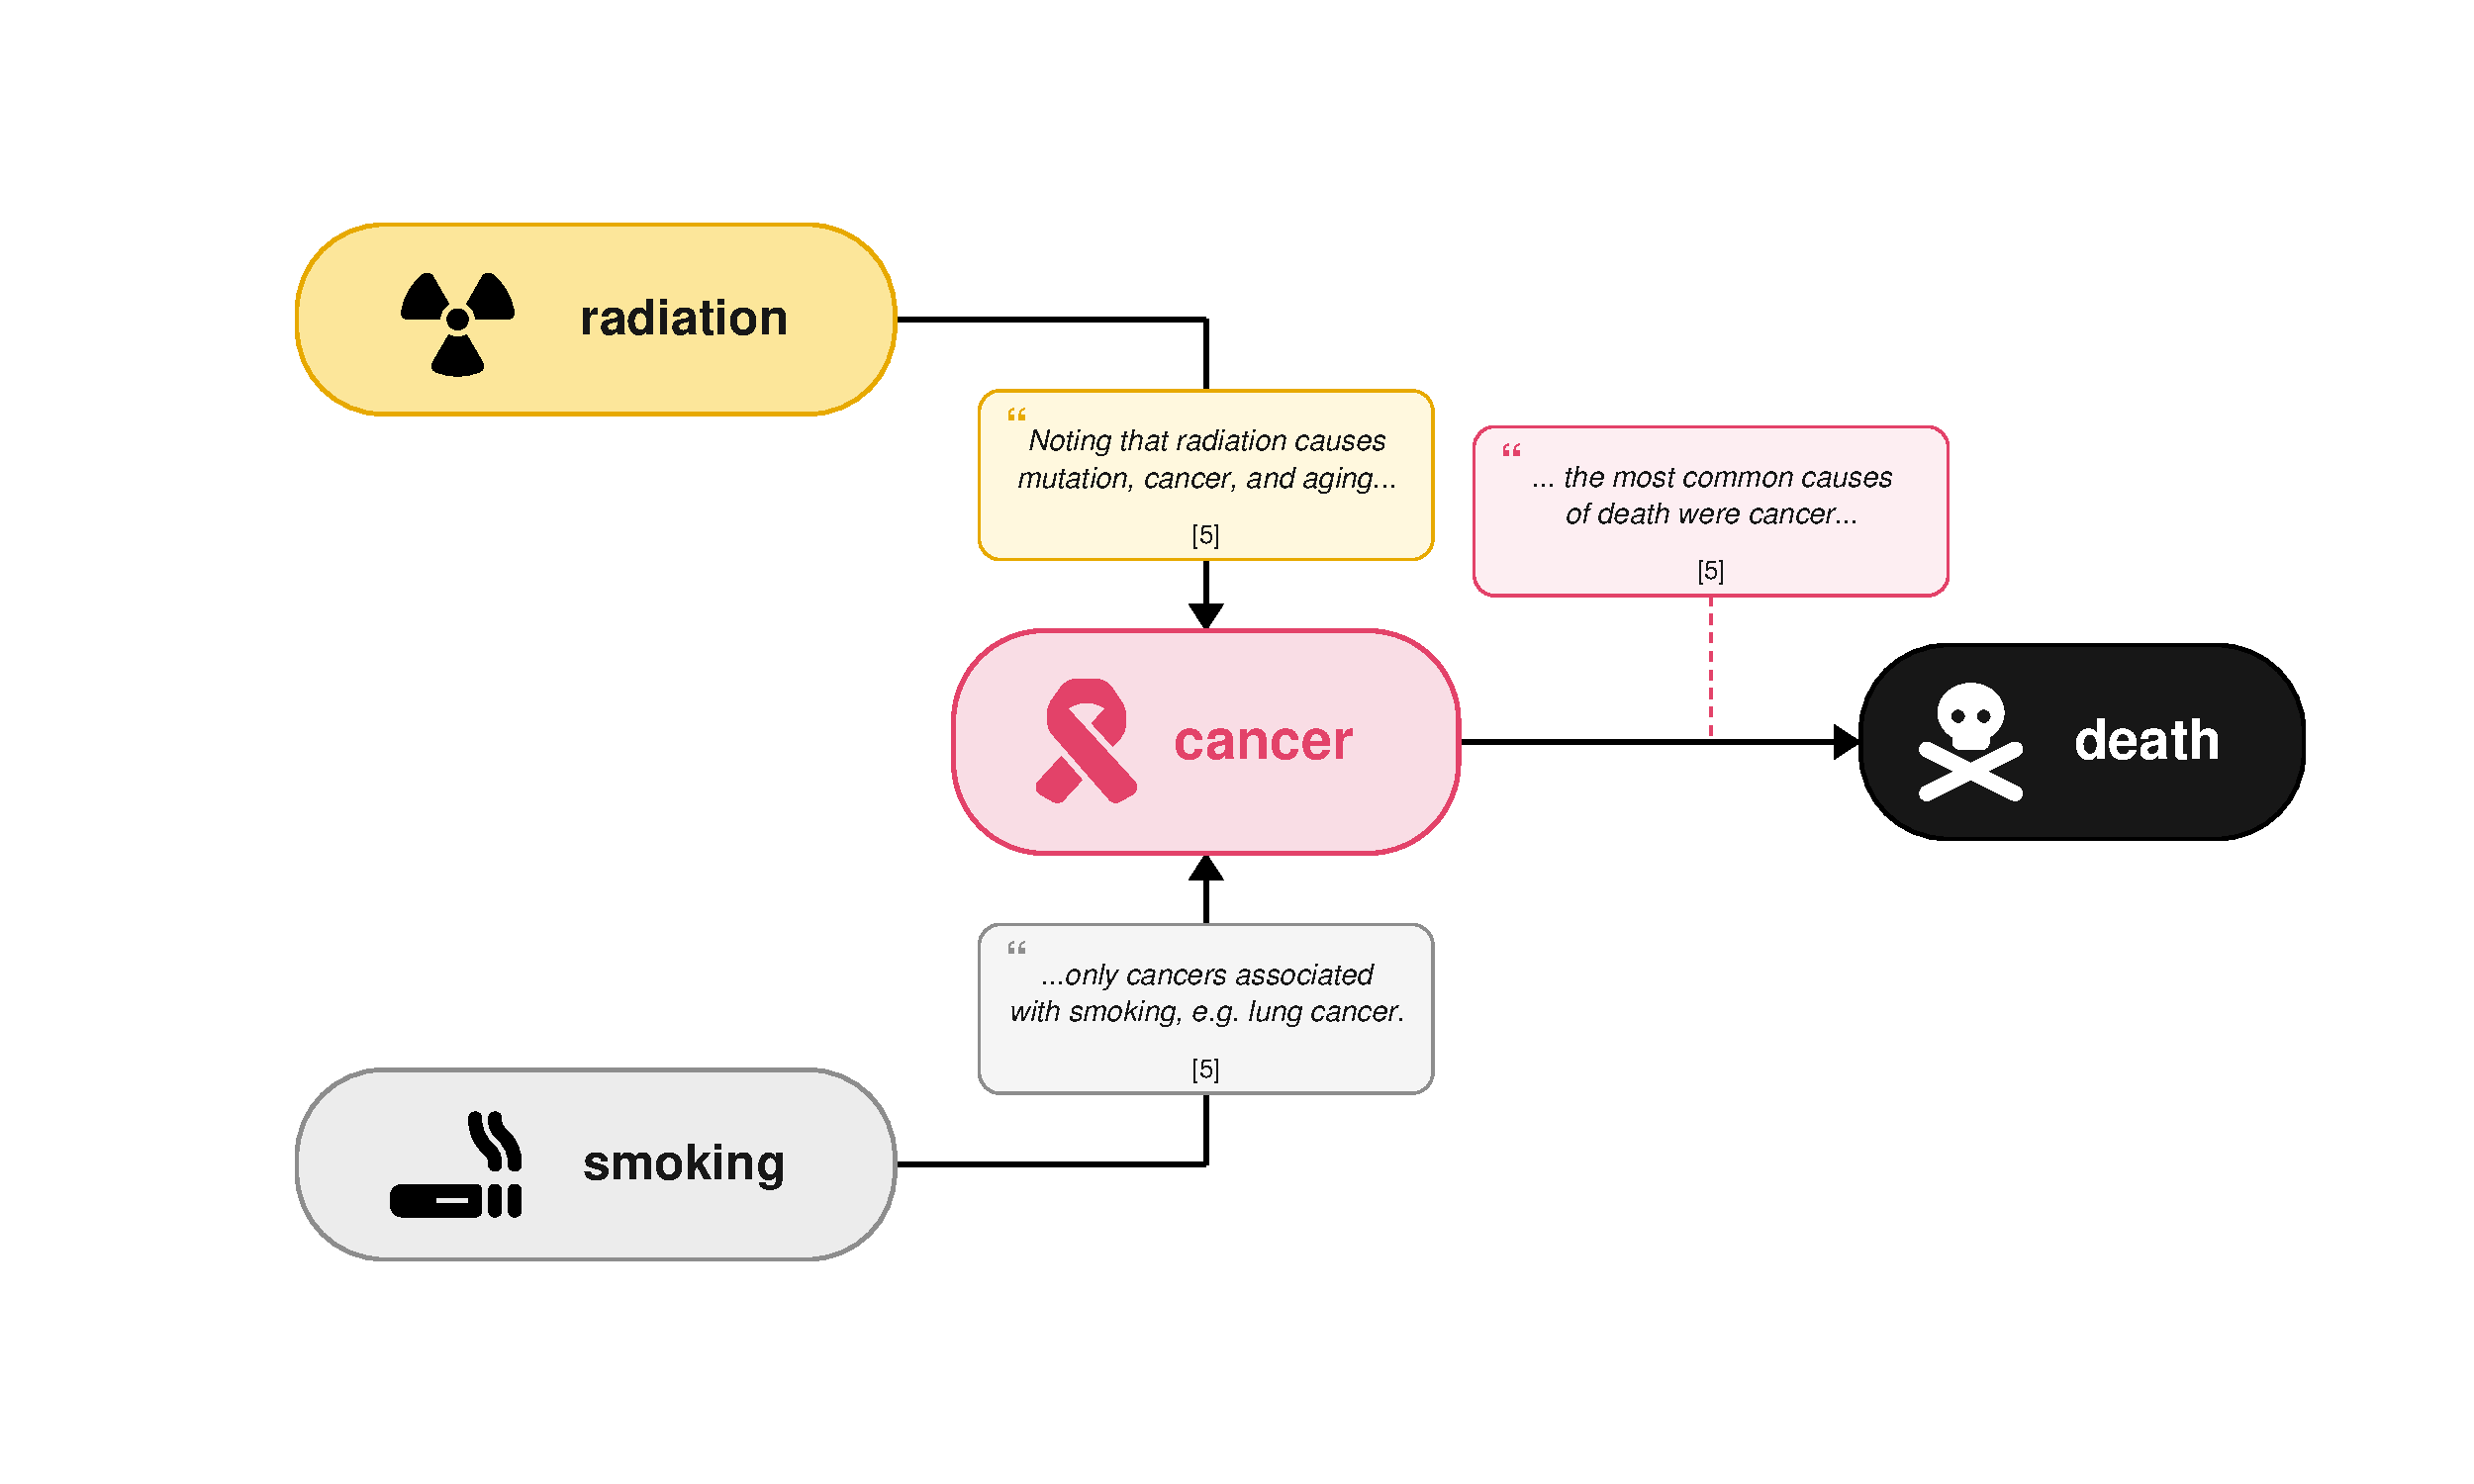
\includegraphics[width=1\linewidth]{figures/causenet.pdf}
    \caption{Example excerpt from CauseNet showing causal relations between concepts such as radiation, smoking, cancer, and death~\cite{heindorf:2020}.}
    \label{fig:causenet_example}
\end{figure}

\subsection{CausalBank and CEG}
\label{sec:rw_causalbank}

\citet{li:2020} introduce two related open-domain causal resources extracted automatically from the English Common Crawl corpus, namely CausalBank and CEG. CausalBank is a sentence-level corpus containing approximately $314$ million cause--effect pairs identified using lexical patterns that explicitly express causal relationships. CEG aggregates these extracted relationships into a directed graph between lemmatized terms. As this thesis investigates graph traversal, it uses CEG rather than the sentence-level CausalBank corpus. Each edge records the occurrence frequency of the corresponding term pair together with necessity and sufficiency causality scores. \citeauthor{li:2020} report approximately $89.1$ million relationships after filtering those occurring five times or less~\cite{li:2020}.

\section{RL Agent for Graph Traversal}
\label{sec:rw_rl}

\citet{bluebaum:2024} propose a reinforcement learning (RL) approach to binary causal question answering through graph traversal. Their agent is trained on CauseNet to learn a policy that maps the query and current graph node to a distribution over neighboring nodes. During inference, multiple paths are sampled, and a causal relationship is predicted if and only if one reaches the target node. By directing traversal toward promising neighbors, the approach reduces the number of explored nodes by up to $99\%$ compared with BFS while maintaining comparable accuracy~\cite{bluebaum:2024}. Despite these gains, the method requires training an RL agent and repeatedly evaluating its policy during traversal, resulting in additional computational overhead.

\section{Learned Heuristics for Search}
\label{sec:rw_learned_heuristics}

Informed search algorithms such as $A^*$ rely on heuristic functions to estimate
the remaining cost from a current state to the goal. Designing effective
heuristics manually often requires substantial domain knowledge and
problem-specific experimentation, which has motivated approaches that learn
these estimates from data. \citet{numeroso:2022} propose a
neural method for learning consistent heuristic functions that can be integrated directly into $A^*$ search. On synthetic pathfinding tasks, their learned heuristics reduce search effort compared with Dijkstra's algorithm while preserving optimality. This thesis instead investigates learned heuristics for binary causal question answering over large-scale causal knowledge graphs.


\chapter{Methodology}
\label{chap:methodology}

This chapter presents the proposed methodology for binary causal question answering over directed causal knowledge graphs. Section~\ref{sec:method_formulation} specifies the graph-based problem setting considered in this work. Section~\ref{sec:method_search} introduces the bounded embedding-guided $A^*$ search procedure, including its traversal cost and heuristic functions. Section~\ref{sec:method_finetuning} motivates the fine-tuning of the embedding space for more effective search guidance. Finally, Section~\ref{sec:method_framework} provides an overview of the main software components and interactive demonstration.

\section{Problem Setting}
\label{sec:method_formulation}

Following the graph-based formulation introduced in Section~\ref{sec:foundations_graphs}, this thesis treats binary causal question answering as directed reachability. Given two concepts $A$ and $B$ with corresponding graph nodes $a,b\in V$, the task is to determine whether a directed path from $a$ to $b$ can be found. A discovered path yields a positive answer, while failure to find one yields a negative answer under the applied search procedure.

\section{Embedding-Guided \texorpdfstring{$A^*$}{A*} Search}
\label{sec:method_search}

To search efficiently for a directed causal path from $a$ to $b$, this work employs an embedding-guided $A^*$ algorithm. In spatial path-finding applications, $A^*$ heuristics often rely on geometric distances, whereas causal knowledge graphs provide no spatial coordinates from which such estimates can be derived. Therefore, each graph node is mapped to a corresponding point in a $d$-dimensional embedding space according to
\[
\phi \colon V \rightarrow \mathbb{R}^{d},
\]
where $\phi(v)$ denotes the vector representation of node $v$. The traversal cost of an edge $(u,v)$ is defined as the distance between the embeddings of $u$ and $v$,
\[
c(u,v)=d\bigl(\phi(u),\phi(v)\bigr),
\]
where $d(\cdot,\cdot)$ denotes either cosine or Euclidean distance. For a node $n$, the accumulated cost from the start node $a$ is defined as
\[
g(n)=\sum_{(u,v)\in P_{a,n}} c(u,v),
\]
where $P_{a,n}$ denotes the currently known path from $a$ to $n$. The heuristic function estimates the remaining distance from $n$ to the target node $b$ as
\[
h(n)=d\bigl(\phi(n),\phi(b)\bigr),
\]
and the priority of each node is determined by
\[
f(n)=g(n)+h(n).
\]
Let $\tau$ denote the maximum visited-node budget, with $\tau=-1$ indicating that no limit is applied. Nodes are expanded in ascending order of $f(n)$ until $b$ is reached, the priority queue is exhausted, or $\tau$ is exceeded. The implementation retains the lowest known path cost for each node and does not reopen nodes after expansion. This reduces traversal overhead but does not retain the optimality guarantee of classical $A^*$ when the heuristic is not consistent. Algorithm~\ref{alg:bounded-astar} presents the proposed bounded embedding-guided $A^*$ search.

\section{Fine-Tuning the Embedding Space}
\label{sec:method_finetuning}

The evaluated pretrained embedding models are designed primarily for semantic similarity, retrieval, or ranking rather than causal graph traversal~\cite{allmpnet:modelcard,bge:modelcard,granite:modelcard,mxbai:modelcard,qwen3:modelcard}. Their original embedding spaces therefore do not necessarily reflect which neighboring nodes are most relevant for reaching a causal target. To improve the search heuristic, the embedding space is fine-tuned using successful causal search paths. At each step, the successor on the discovered path is contrasted with alternative outgoing neighbors, encouraging the model to assign more favorable embedding-space distances to transitions that lead toward the target. The resulting representations are therefore better aligned with the requirements of embedding-guided $A^*$ search. Chapter~\ref{chap:train} details this procedure.

\section{Implementation Overview}
\label{sec:method_framework}

The implementation covers graph search, hyperparameter optimization, model training, evaluation, and interactive visualization. Dataset processing relies on Hugging Face Datasets~\cite{lhoest:2021}, while Optuna~\cite{akiba:2019} is used to optimize the hyperparameters before training. The Sentence Transformer models~\cite{reimers:2019} are subsequently trained with PyTorch~\cite{paszke:2019} and PyTorch Lightning~\cite{falcon:2019}, while NumPy~\cite{harris:2020} is used for embedding storage and access. The demonstration shown in Figure~\ref{fig:frontend-demo} is implemented using FastAPI~\cite{ramirez:fastapi} and 3d-force-graph~\cite{asturiano:3dforcegraph}. It allows users to select a graph, embedding model, and Matryoshka dimension, execute embedding-guided $A^*$ search, and visualize the resulting causal path.\footnote{The demonstration is deployed at \url{https://pathfinding.demo.causenet.org}.}

\begin{figure}[t]
    \centering
    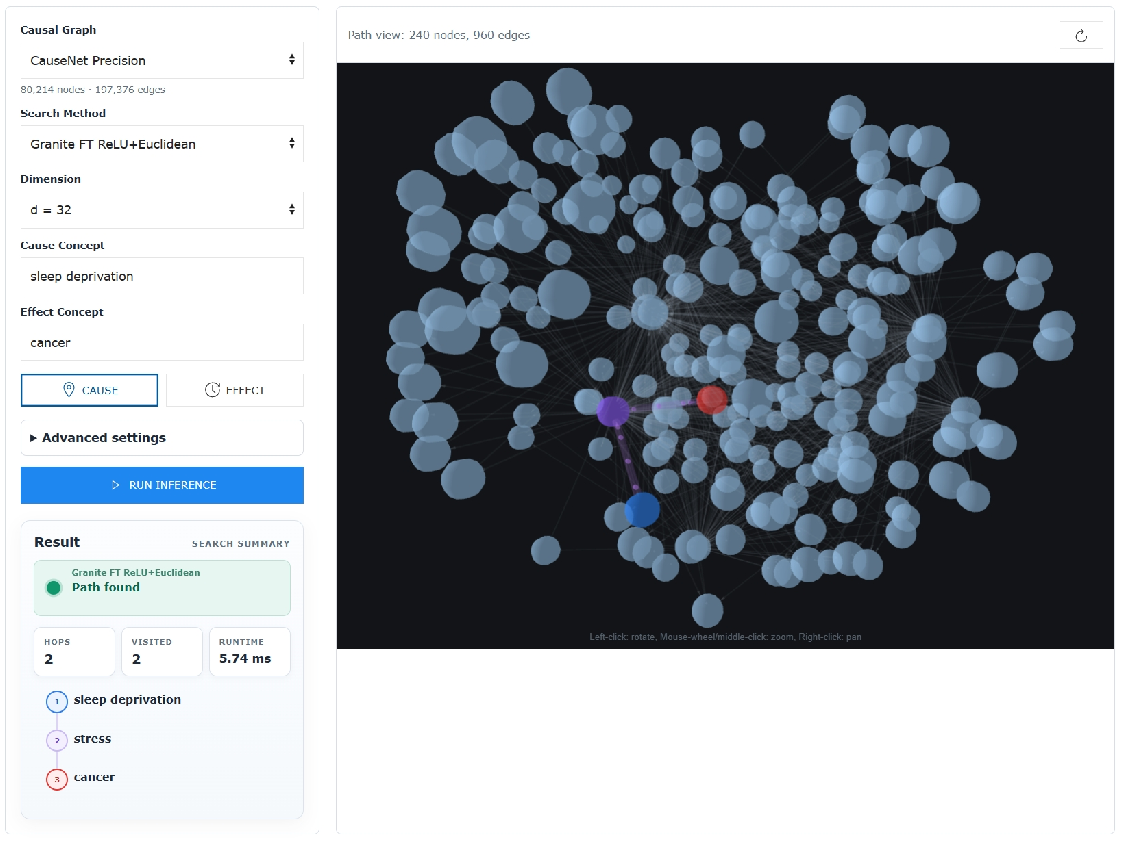
\includegraphics[width=\textwidth]{figures/app.pdf}
    \caption{Web interface for configuring embedding-guided $A^*$ search and visualizing the resulting causal path.}
    \label{fig:frontend-demo}
\end{figure}

\chapter{Training Procedure}
\label{chap:train}

This chapter describes the procedure used to adapt pretrained embedding models for more efficient $A^*$ traversal. Section~\ref{sec:train_dataset} explains how successful graph traversals are converted into supervised preference examples. Sections~\ref{sec:train_objective} and~\ref{sec:train_matryoshka} introduce the ranking-based training objective and its extension to Matryoshka Representation Learning. Section~\ref{sec:train_validation} presents the search-based validation procedure, while Sections~\ref{sec:train_hyperparameters} and~\ref{sec:train_final_training} describe hyperparameter optimization and final model training. Finally, Section~\ref{sec:train_final_precomputation} explains how the trained embeddings are precomputed and stored for evaluation and inference.

\section{Supervision Construction}
\label{sec:train_dataset}

To fine-tune the embedding models, supervised training and validation datasets are constructed from the corresponding splits of the binary causal question dataset derived from MS MARCO by \citet{bluebaum:2024}. This construction is specific to model training and hyperparameter optimization, while the subsequent evaluation data remain unchanged. Each pretrained base model is used to generate its own supervision.

To construct a dataset for a given split, consider a causal graph $G=(V,E)$. Graph-node embeddings are first precomputed using the respective pretrained base model. For each cause--effect pair $(A,B)$ in the split, let $a,b\in V$ denote the corresponding graph nodes. An unbounded $A^*$ search is performed from \mbox{$a$ to $b$} using distance metric $d\in\{\mathrm{Cos},\mathrm{Euc}\}$, denoting cosine and Euclidean distance, respectively. If the search reaches the target $b$, the discovered path is retained. Let
\[
P=(p_0,\dots,p_k), \qquad p_0=a,\quad p_k=b,\quad k\geq1,
\]
denote such a path, where $p_i$ is the node at position $i$ and $k$ is the number of edges in the path. The $A^*$ path is used instead of a minimum-hop path obtained with BFS because minimizing the number of edges does not necessarily yield a path useful for embedding-guided search. In contrast, $A^*$ prioritizes nodes according to the embedding-space edge costs and heuristic estimates of the pretrained model. The resulting paths therefore provide supervision aligned with the search procedure that fine-tuning aims to improve.

For each distance metric $d$, let $\mathcal{D}_{\mathrm{train}}^d$ and $\mathcal{D}_{\mathrm{val}}^d$ denote the datasets constructed from the training and validation splits, respectively. Let $N^+(p_i)$ denote the set of outgoing successors of node $p_i$. For every step along a retained path, the path successor $p_{i+1}$ is treated as the preferred choice and compared with each alternative successor $n\in N^+(p_i)\setminus\{p_{i+1}\}$. For either split $s\in\{\mathrm{train},\mathrm{val}\}$, the corresponding quadruples are added as
\[
\mathcal{D}_s^d \gets \mathcal{D}_s^d \cup
\left\{
(p_i,p_k,p_{i+1},n)
\;\middle|\;
0\leq i<k,\;
n\in N^+(p_i)\setminus\{p_{i+1}\}
\right\}.
\]
Each quadruple is subsequently denoted by $(c,e,p,n)$, representing the current node, target node, preferred successor on the discovered path, and alternative successor, respectively. It defines a pairwise preference that encourages the model to assign a lower estimated traversal cost to the preferred successor than to the competing choice. Algorithm~\ref{alg:training-dataset} summarizes the construction procedure. The resulting datasets are cached after construction and reused throughout hyperparameter optimization and final model training, avoiding repeated $A^*$ searches for generating the same supervision.


\section{Ranking-Based Training Objective}
\label{sec:train_objective}

The ranking-based objective uses quadruples $(c,e,p,n)\in \mathcal{D}_{\mathrm{train}}^d$ to reshape the embedding space for graph traversal. The preferred successor $p$ should yield a lower cumulative distance to the target $e$ than the alternative successor $n$. The difference between the preferred and alternative traversal costs is defined as\looseness=-1
\[
\begin{aligned}
\Delta &= f(p)-f(n) \\
&= \bigl[g(p)+h(p)\bigr]-\bigl[g(n)+h(n)\bigr] \\
&=
\left[
d\bigl(\phi(c),\phi(p)\bigr)
+
d\bigl(\phi(p),\phi(e)\bigr)
\right]
-
\left[
d\bigl(\phi(c),\phi(n)\bigr)
+
d\bigl(\phi(n),\phi(e)\bigr)
\right].
\end{aligned}
\]
A value $\Delta<0$ indicates that the preferred traversal decision is favored. The ranking loss is obtained by applying a non-linear activation function $\sigma$ to $\Delta$
\[
\mathcal{L}_{\mathrm{rank}}=\sigma(\Delta).
\]
This work evaluates ReLU and GELU as activation functions. An additional regularization term encourages the embedding norms to remain close to one
\[
\mathcal{L}_{\mathrm{reg}}
=
\sum_{x\in\{c,e,p,n\}}
\left(\lVert\phi(x)\rVert_2-1\right)^2.
\]
For a single embedding dimension, the resulting loss is
\[
\mathcal{L}
=
\mathcal{L}_{\mathrm{rank}}+\mathcal{L}_{\mathrm{reg}}.
\]
The objective therefore optimizes embedding distances for causal graph traversal rather than semantic similarity.


\section{Matryoshka Representation Learning}
\label{sec:train_matryoshka}

To support efficient causal knowledge graph traversal at different embedding dimensions, the ranking objective is extended using Matryoshka Representation Learning~\cite{kusupati:2022}. Rather than optimizing only the full embedding vector, the objective is applied to multiple nested prefixes of each representation. Let $D_{\mathrm{model}}$ denote the native embedding dimensionality of the underlying model. The set of training dimensions is defined as
\[
\mathcal{M}
=
\{D_{\mathrm{model}}\}
\cup
\left\{
2^k
\;\middle|\;
k\in\mathbb{N},\;
2\leq 2^k<D_{\mathrm{model}}
\right\}.
\]
The dimension 768 is additionally included in $\mathcal{M}$ to enable direct comparison with MPNet and Granite, whose native dimensionality is 768~\cite{allmpnet:modelcard,granite:modelcard}.
\[
\mathcal{M}\gets\mathcal{M}\cup\{768\}.
\]
For each $m\in\mathcal{M}$, let
\[
\phi_m(x)=\phi(x)_{1:m}
\]
denote the first $m$ components of the embedding of concept $x$. Let $f_m$, $g_m$, and $h_m$ denote the corresponding $A^*$ evaluation, path-cost, and heuristic terms computed using $\phi_m$. The corresponding evaluation difference is
\[
\begin{aligned}
\Delta_m &= f_m(p)-f_m(n) \\
&= \bigl[g_m(p)+h_m(p)\bigr]-\bigl[g_m(n)+h_m(n)\bigr] \\
&=
\left[
d\bigl(\phi_m(c),\phi_m(p)\bigr)
+
d\bigl(\phi_m(p),\phi_m(e)\bigr)
\right]
\\
&\phantom{=}
-
\left[
d\bigl(\phi_m(c),\phi_m(n)\bigr)
+
d\bigl(\phi_m(n),\phi_m(e)\bigr)
\right].
\end{aligned}
\]
The dimension-specific ranking loss is
\[
\mathcal{L}_{\mathrm{rank}}^{(m)}
=
\sigma(\Delta_m).
\]
The overall training loss is
\[
\mathcal{L}_{\mathrm{total}}
=
\sum_{m\in\mathcal{M}}
\mathcal{L}_{\mathrm{rank}}^{(m)}
+
\mathcal{L}_{\mathrm{reg}}.
\]
Thus, every Matryoshka prefix contributes a ranking loss, while the norm regularization remains global. Applying the objective at multiple prefix lengths encourages information relevant to causal graph traversal to be concentrated in the earlier embedding dimensions. This enables a single fine-tuned model to support multiple embedding dimensions without additional training, allowing the representation size to be selected according to the desired trade-off between computational efficiency and heuristic quality.


\section{Validation Procedure}
\label{sec:train_validation}

Although the training objective optimizes local ranking decisions, validation measures whether the learned embedding space improves global graph traversal. At the beginning of each validation epoch, embeddings for all graph nodes are recomputed using the current state of the model and stored in a temporary lookup cache. For each distinct pair $(c,e)$ occurring in the supervision dataset $\mathcal{D}_{\mathrm{val}}^d$ within a validation batch, an $A^*$ search is performed from the current node $c$ to the target node $e$ using these updated embeddings and distance metric $d$. The number of nodes visited before reaching the target is recorded as $v(c,e)$. Let $P_{\mathrm{val}}^d$ denote the collection of evaluated pairs after batch-wise deduplication. The primary validation metric is the average number of visited nodes
$$
\text{AvgVisited}
=
\frac{1}{|P_{\mathrm{val}}^d|}
\sum_{(c,e)\in P_{\mathrm{val}}^d}
v(c,e).
$$
Lower values indicate that fewer graph nodes are visited on average before reaching the target and therefore correspond to more efficient traversal.


\section{Hyperparameter Optimization}
\label{sec:train_hyperparameters}

Before final training, model-specific hyperparameter optimization is performed with Optuna~\cite{akiba:2019}. The search jointly optimizes the learning rate, activation function (ReLU or GELU), and distance metric (cosine or Euclidean) using the Tree-structured Parzen Estimator sampler~\cite{bergstra:2011}. The learning rate is sampled logarithmically from $[2.5 \times 10^{-5}, 3 \times 10^{-5}]$. This interval was selected based on preliminary experiments indicating stable and competitive validation performance within this range. Each trial performs a short training run and is evaluated by the average number of nodes visited during validation $A^*$ searches. Early stopping terminates training when this metric no longer improves~\cite{prechelt:1998}, while Optuna's MedianPruner stops trials that underperform the median result of previously completed trials at the same training step~\cite{optuna:medianpruner}. For each embedding model, hyperparameter optimization first runs 30 completed or pruned trials and then continues one trial at a time. The search stops after five consecutive trials without a lower average number of visited nodes on validation. An improvement resets this counter, allowing up to 50 trials. Each trial runs for at most 10 epochs with an early-stopping patience of 3 validation epochs. Training uses the AdamW optimizer~\cite{loshchilov:2019} and a \mbox{ReduceLROnPlateau} scheduler~\cite{pytorch:reducelronplateau}, which halves the learning rate after one validation epoch without improvement. The effective batch size is fixed at 128, using gradient accumulation for smaller physical batches~\cite{ott:2018,lightning:gradientaccumulation}.

\section{Final Model Training}
\label{sec:train_final_training}

After hyperparameter optimization, the configuration with the lowest average number of visited nodes is selected for each embedding model. Final training uses the selected learning rate, activation function, and distance metric for up to 50 epochs with early stopping and a patience of 10 validation epochs. The checkpoint with the lowest average number of visited nodes on the validation set is retained as the final model and saved together with its training metadata.

\section{Final Embedding Precomputation}
\label{sec:train_final_precomputation}

After training, embeddings are precomputed for all graph-node concepts required during evaluation and inference. The node concepts are stored in a fixed order in a shared JSONL file. All embedding matrices follow this same ordering, allowing each node concept to be mapped to its row index and its embedding to be retrieved directly from the corresponding memory-mapped NumPy matrix~\cite{harris:2020}. The model first produces embeddings at its native dimensionality. For every Matryoshka dimension used in the experiments, the corresponding prefix of each full embedding is stored in a separate matrix. During graph traversal, $A^*$ loads the matrix for the selected model and dimension instead of computing embeddings with the encoder at runtime. This reduces inference time and enables direct indexed access to all node embeddings. The approach therefore trades additional disk space for lower runtime.


\chapter{Results}
\label{chap:results}

This chapter evaluates the proposed embedding-guided $A^*$ search for binary causal question answering, focusing on both effectiveness and search efficiency. The evaluation addresses four research questions. RQ1 assesses the impact of fine-tuning on the embedding heuristic, while RQ2 analyzes the role of Matryoshka dimensionality. RQ3 compares the selected $A^*$ configuration with the BFS and RL baselines. Finally, RQ4 evaluates its generalization across different datasets and causal graph variants.

Section~\ref{sec:results-evaluation-setup} introduces the experimental setup and evaluation metrics. The subsequent analyses examine the effect of fine-tuning in Section~\ref{sec:results-finetuning} and Matryoshka dimensionality in Section~\ref{sec:results-matryoshka}, addressing RQ1 and RQ2, respectively. Section~\ref{sec:results-comparison} presents the final comparison with the baselines and evaluates performance across datasets and graph variants, addressing RQ3 and RQ4. Finally, Section~\ref{sec:results-ablation} concludes the analysis with an ablation study of the activation function and distance metric.

\section{Evaluation Setup}
\label{sec:results-evaluation-setup}

This section describes the evaluation procedure, datasets, causal graphs, models and baselines, and the methodology used throughout the experiments.

\subsection{Evaluation Procedure}
\label{sec:results-procedure}

The evaluation is organized in two stages. First, MS MARCO validation~\citep{nguyen:2016,bluebaum:2024} with CauseNet Precision~\citep{heindorf:2020} is used to analyze fine-tuning and Matryoshka dimensionality and select the final $A^*$ configuration. Second, the selected configuration is evaluated on the MS MARCO and SemEval~\citep{hendrickx:2010,sharp:2016,bluebaum:2024} test splits across CauseNet Precision, CauseNet Full~\citep{heindorf:2020}, and CEG Filtered~\citep{li:2020}, and compared with BFS and the RL approach of \citet{bluebaum:2024}.

\subsection{Datasets}
\label{sec:results-datasets}

The causal question answering datasets used in this thesis are derived subsets rather than the complete original datasets. The MS MARCO data are based on causal questions extracted from the original MS MARCO dataset~\citep{nguyen:2016} as part of Webis-CausalQA-22~\citep{bondarenko:2022}, while the SemEval data are based on the causal-relation subset of SemEval-2010 Task 8~\citep{hendrickx:2010} introduced by \citet{sharp:2016}. The binary causal splits for both datasets were provided by \citet{bluebaum:2024}. During evaluation, examples are skipped if the potential cause, the effect, or both are absent from the evaluated graph. Table~\ref{tab:dataset-statistics} reports the dataset sizes and class distributions in the original splits and after graph-node coverage filtering. Because graph-node coverage differs across graphs, each graph is evaluated on a different subset of questions with a different class distribution. Differences in effectiveness across graphs should therefore not be attributed solely to the graph itself.

\begin{table}[t]
\centering
\small
\setlength{\tabcolsep}{6pt}
\caption{Number of causal questions in MS MARCO and SemEval before and after graph-node coverage filtering. ``Total'' counts all causal samples in each local split. The graph columns count samples where both the potential cause and effect are covered by the corresponding graph.}
\label{tab:dataset-statistics}
\begin{tabular}{@{}p{2.75cm}rrrrrrrr@{}}
\toprule
\textbf{Split}
& \multicolumn{2}{c}{\textbf{Total}}
& \multicolumn{2}{c}{\textbf{CauseNet\textsubscript{Prec}}}
& \multicolumn{2}{c}{\textbf{CauseNet\textsubscript{Full}}}
& \multicolumn{2}{c}{\textbf{CEG\textsubscript{Filtered}}} \\
\cmidrule(lr){2-3}
\cmidrule(lr){4-5}
\cmidrule(lr){6-7}
\cmidrule(l){8-9}
& \textbf{Pos.} & \textbf{Neg.}
& \textbf{Pos.} & \textbf{Neg.}
& \textbf{Pos.} & \textbf{Neg.}
& \textbf{Pos.} & \textbf{Neg.} \\
\midrule
\multicolumn{9}{@{}l}{MS MARCO \citep{nguyen:2016,bluebaum:2024}} \\
Train      & $1{,}837$ & $0$  & $1{,}213$ & $0$  & $1{,}618$ & $0$  & $389$ & $0$ \\
Validation & $194$     & $47$ & $137$     & $22$ & $176$     & $35$ & $44$  & $8$ \\
Test       & $223$     & $40$ & $143$     & $20$ & $189$     & $31$ & $41$  & $7$ \\
\addlinespace[2pt]
\multicolumn{9}{@{}l}{SemEval \citep{hendrickx:2010,sharp:2016,bluebaum:2024}} \\
Train      & $694$ & $690$ & $541$ & $177$ & $680$ & $615$ & $496$ & $416$ \\
Validation & $84$  & $89$  & $66$  & $28$  & $81$  & $77$  & $57$  & $65$ \\
Test       & $87$  & $86$  & $66$  & $24$  & $84$  & $76$  & $57$  & $53$ \\
\bottomrule
\end{tabular}
\end{table}


\subsection{Causal Graphs}
\label{sec:results-graphs}

The evaluation uses three graph settings. CauseNet Precision is the high-precision subset of CauseNet~\citep{heindorf:2020} and is used for training, validation, model selection, and the main comparison to prior work. CauseNet Full is used to test scalability to a substantially larger graph. The third evaluated graph is a filtered version of the original CEG~\citep{li:2020}. Because CEG is very dense and contains many low-confidence edges, filtering is applied using the causal-strength formulation of \citet{luo:2016}, which combines necessity and sufficiency scores. For each CEG edge from cause \(c\) to effect \(e\), the causal strength is computed as\looseness=-1
\[
    \mathrm{CS}(c,e)
    =
    \mathrm{necessity}(c,e)^{\lambda}
    \cdot
    \mathrm{sufficiency}(c,e)^{1-\lambda},
\]
where \(\lambda\in[0,1]\) is a weighting parameter. This thesis uses \(\lambda = 0.9\), following \citeauthor{luo:2016}, and retains only edges with \(\mathrm{CS}(c,e) \geq 0.1\). All graph files undergo the same preprocessing, which removes empty or punctuation-only concepts and self-loops and normalizes labels by replacing underscores with spaces and stripping surrounding whitespace. Table~\ref{tab:graph-statistics} reports the resulting graph sizes.\footnote{The publicly available CEG release, in which cause--effect pairs with a reported frequency of \(5\) or lower are already excluded, contains approximately \(92.3\) million edges. In contrast, the official CEG release documentation~\citep{li:2020} reports approximately \(89.1\) million cause--effect pairs for this version. The available release information is insufficient to determine the source of this discrepancy conclusively. The official CauseNet statistics report \(199{,}806\) relations and \(80{,}223\) concepts for CauseNet Precision and \(11{,}609{,}890\) relations and \(12{,}186{,}195\) concepts for CauseNet Full~\citep{heindorf:2020}. The slightly smaller counts in Table~\ref{tab:graph-statistics} result from the preprocessing used in this thesis, which removes empty or punctuation-only concepts and self-loops and normalizes concept labels.}

\begin{table}[t]
  \centering
  \small
  \begin{tabular}{@{}p{9.65cm}rr@{}}
    \toprule
    \textbf{Graph} & \textbf{Nodes} & \textbf{Edges} \\
    \midrule
    CauseNet Precision & $80{,}211$ & $197{,}370$ \\
    CauseNet Full & $12{,}185{,}890$ & $11{,}606{,}919$ \\
    CEG Filtered & $77{,}264$ & $21{,}507{,}177$ \\
    CEG & $79{,}865$ & $92{,}270{,}736$ \\
    \bottomrule
  \end{tabular}
  \caption{Number of nodes and unique directed edges after graph preprocessing. CEG is reported for reference, while CEG Filtered is used in the evaluation.}
  \label{tab:graph-statistics}
\end{table}


\subsection{Models and Baselines}
\label{sec:results-models}

For embedding-guided \(A^*\), five embedding backbones are evaluated alongside the RL baseline of \citet{bluebaum:2024}. The \(A^*\) models and RL policy are trained using the MS MARCO training split and CauseNet Precision. Unlike the original RL setup, the policy is trained and evaluated without inverse edges because these may introduce transitions that do not represent causality in the queried direction. This ensures that all methods operate on the same forward directed-reachability task. Table~\ref{tab:model-overview} defines the model identifiers, parameter counts, embedding dimensions, and concise labels used throughout the results. Table~\ref{tab:training-hyperparameters} reports the selected hyperparameters and final training epoch for each fine-tuned embedding model. The epoch denotes the zero-indexed last validation improvement before early stopping with a patience of 10. The checkpoint from this epoch is retained as the final model.


\begin{table}[t]
\centering
\footnotesize
\setlength{\tabcolsep}{4pt}
\caption{Models used in the evaluation. The table reports the model labels used throughout this thesis, the corresponding model identifiers, parameter counts, and native embedding dimensions $d$.}
\label{tab:model-overview}
\begin{tabular}{@{}p{3.55cm}p{7.45cm}r r@{}}
\toprule
\textbf{Model label} & \textbf{Model identifier} & \textbf{Params.} & $\boldsymbol{d}$ \\
\midrule
RL \citep{bluebaum:2024}
& LSTM policy model
& 12M & -- \\

MPNet \citep{song:2020mpnet,allmpnet:modelcard}
& \texttt{sentence-transformers/all-mpnet-base-v2}
& 109M & 768 \\

BGE \citep{xiao:2024,bge:modelcard}
& \texttt{BAAI/bge-large-en-v1.5}
& 335M & 1024 \\

Granite \citep{awasthy:2025graniter2,granite:modelcard}
& \texttt{ibm-granite/granite-embedding-english-r2}
& 149M & 768 \\

mxbai \citep{mixedbread:2024mxbai,mxbai:modelcard}
& \texttt{mixedbread-ai/mxbai-embed-large-v1}
& 335M & 1024 \\

Qwen \citep{zhang:2025qwen3embedding,qwen3:modelcard}
& \texttt{Qwen/Qwen3-Embedding-0.6B}
& 0.6B & 1024 \\
\bottomrule
\end{tabular}
\end{table}

\begin{table}[t]
  \centering
  \small
  \begin{tabular}{@{}c@{\hspace{7.25em}}c@{}}
    \textbf{(a) Selected hyperparameters} & \textbf{(b) Selected epoch} \\[2pt]
    \begin{tabular}[t]{@{}lllr@{}}
      \toprule
      \textbf{Model} & \textbf{Activation} & \textbf{Metric} & \textbf{lr [$10^{-5}$]} \\
      \midrule
      MPNet & ReLU & Cosine & $2.673$ \\
      BGE & ReLU & Cosine & $2.924$ \\
      mxbai & ReLU & Cosine & $2.935$ \\
      Granite & ReLU & Euclidean & $2.709$ \\
      Qwen & ReLU & Cosine & $2.887$ \\
      \bottomrule
    \end{tabular}
    &
    \begin{tabular}[t]{@{}lr@{}}
      \toprule
      \textbf{Model} & \textbf{Epoch} \\
      \midrule
      MPNet & 0 \\
      BGE & 0 \\
      mxbai & 3 \\
      Granite & 10 \\
      Qwen & 10 \\
      \bottomrule
    \end{tabular}
  \end{tabular}
  \caption{Final training settings. Panel (a) reports the selected activation function, distance metric, and learning rate. Panel (b) reports the zero-indexed epoch of the last improvement in validation $A^*$ cost. Its checkpoint is retained for evaluation.}
  \label{tab:training-hyperparameters}
\end{table}


\subsection{Evaluation Methodology}
\label{sec:results-methodology}

This section describes the experimental evaluation, including search budgets, metrics, runtime measurement, model selection, and significance testing.

\subsubsection{Search Budgets}

The evaluation reports two BFS variants and budgeted \(A^*\). BFS (uncapped) runs without a visit limit and serves as the exhaustive reachability baseline. For BFS (capped) and \(A^*\), budgets are set to the 95th percentile ($p_{95}$) of visited nodes from successful searches on the MS MARCO training split with CauseNet Precision. BFS uses one global cap, whereas \(A^*\) uses separate budgets for each embedding model and Matryoshka dimension, as reported in Table~\ref{tab:p95-visited-nodes}. Uncapped \(A^*\) is additionally reported in the fine-tuning analysis to separate the effect of fine-tuning from the visit budget. The Matryoshka and final evaluations use the budgeted variants. Following the implementation of \citet{bluebaum:2024}, RL has no visit budget and instead uses beam search with a beam width of \(50\), a \textsc{stay} action, and a rollout length of two.

\begin{table}[H]
\centering
\small
\caption{$A^*$ visit budgets $\tau$ derived from the $p_{95}$ of visited nodes in successful searches on MS MARCO train with CauseNet Precision. Pretrained models are reported at their full embedding dimension, while fine-tuned models are reported across all evaluated Matryoshka dimensions.}
\label{tab:p95-visited-nodes}
\begin{tabular}{@{}p{2.39cm}rrrrrrrrrrr@{}}
\toprule
\textbf{Model} & \multicolumn{11}{c}{\textbf{Dimension}} \\
\cmidrule(l){2-12}
 & \textbf{2} & \textbf{4} & \textbf{8} & \textbf{16} & \textbf{32} & \textbf{64} & \textbf{128} & \textbf{256} & \textbf{512} & \textbf{768} & \textbf{1024} \\
\midrule
BGE & -- & -- & -- & -- & -- & -- & -- & -- & -- & -- & $379$ \\
BGE tuned & $682$ & $96$ & $27$ & $12$ & $10$ & $8$ & $8$ & $8$ & $9$ & $10$ & $10$ \\

Granite & -- & -- & -- & -- & -- & -- & -- & -- & -- & $825$ & -- \\
Granite tuned & $68$ & $16$ & $12$ & $13$ & $16$ & $23$ & $25$ & $23$ & $29$ & $32$ & -- \\

MPNet & -- & -- & -- & -- & -- & -- & -- & -- & -- & $503$ & -- \\
MPNet tuned & $1{,}120$ & $178$ & $41$ & $18$ & $13$ & $14$ & $15$ & $17$ & $21$ & $22$ & -- \\

mxbai & -- & -- & -- & -- & -- & -- & -- & -- & -- & -- & $376$ \\
mxbai tuned & $247$ & $62$ & $20$ & $12$ & $9$ & $8$ & $9$ & $9$ & $9$ & $9$ & $9$ \\

Qwen & -- & -- & -- & -- & -- & -- & -- & -- & -- & -- & $594$ \\
Qwen tuned & $253$ & $105$ & $10$ & $6$ & $5$ & $5$ & $5$ & $5$ & $5$ & $6$ & $5$ \\
\bottomrule
\end{tabular}
\end{table}


\subsubsection{Metrics}

Effectiveness is measured using precision, recall, and F\textsubscript{1}. Efficiency is measured using the average number of visited nodes and the average runtime per query in milliseconds. For BFS and \(A^*\), visited nodes count nodes processed during graph search, whereas for RL, following the original implementation, they count unique nodes in retained beam paths until the target is first encountered. Runtime additionally reflects neural inference, distance computation, and implementation overhead, whereas visited nodes provide a hardware-independent measure of traversal effort that is less sensitive to system load and hardware variation. The two metrics therefore capture complementary aspects of algorithmic search effort and practical execution cost.

\subsubsection{Runtime Measurement}

All evaluations were run on the Webis Slurm infrastructure using eight CPU cores, 128\,GB of memory, and one \texttt{H100} GPU.\footnote{Further details are available at \url{https://webis.de/facilities.html}.} Embedding computations use CUDA, while BFS runs on the CPU. Runtime is measured per query using Python's \texttt{time.perf\_counter()}, with CUDA synchronization before and after traversal. One untimed warm-up is performed per strategy. Graph loading, embedding precomputation, and cache loading are excluded, and reported runtimes are averages over a single evaluation run.

\subsubsection{Model Selection}

The final \(A^*\) configuration is selected from the capped fine-tuned validation results across all Matryoshka dimensions by balancing effectiveness and search efficiency. First, candidates dominated by another configuration with at least as high an F\textsubscript{1} score and no more visited nodes \(N\) are removed. Among the remaining candidates, a knee is selected, representing a point beyond which improving one objective requires a disproportionate deterioration in the other~\citep{branke:2004}. The selection adapts the normalized difference-curve construction of \citet{satopaa:2011}. F\textsubscript{1} and the logarithm of \(N\) are min--max normalized to $\widetilde{F_1}$ and $\widetilde{\log N}$, respectively. The score $(\widetilde{F_1}-\widetilde{\log N})/\sqrt{2}$ measures the signed perpendicular distance from the equal-trade-off diagonal, with larger values indicating a better combination of high F\textsubscript{1} and low search effort. The configuration with the largest score is selected. Runtime, the visit budget, and the embedding dimension are used only as tie-breakers, in that order.

\subsubsection{Statistical Significance Testing}

Statistical significance is tested only for the final test comparison. For each dataset--graph combination, the selected \(A^*\) configuration is compared with BFS (uncapped), BFS (capped), and RL using a paired stratified bootstrap test \citep{koehn:2004,dror:2018}. Positive and negative examples are resampled separately over \(10{,}000\) bootstrap samples. Bonferroni correction is applied to the three comparisons at a family-wise significance level of \(\alpha=0.05\). The reported p-values are Bonferroni-adjusted and compared with \(0.05\), whereas the 95\% confidence intervals remain unadjusted for each individual comparison.

\section{Effect of Fine-Tuning}
\label{sec:results-finetuning}

RQ1 asks whether fine-tuning improves the embedding heuristic used by $A^*$. Table~\ref{tab:validation-full-dim} compares each model before and after fine-tuning at its full embedding dimension on MS MARCO validation with CauseNet Precision, using the best hyperparameter configuration from Table~\ref{tab:training-hyperparameters}. The BFS variants and RL are included as references. RL appears only in the uncapped group because it has no visit budget, although its beam width and rollout length remain fixed. The capped runs use their respective $p_{95}$ budgets from MS MARCO train, whereas the uncapped runs remove the visit limit.

With the cap, pretrained embeddings reach F\textsubscript{1} scores between \(86.2\%\) and \(87.1\%\) while visiting 66.1 to 142.0 nodes on average. Fine-tuning reduces average visited nodes to between 3.5 and 11.0 and runtime for every model, but also lowers F\textsubscript{1} to between \(74.6\%\) and \(82.4\%\). Without the cap, all $A^*$ variants obtain the same F\textsubscript{1} of \(90.6\%\), as uncapped $A^*$ is complete. Fine-tuning nevertheless reduces visited nodes for all five models and runtime for BGE, Granite, MPNet, and Qwen. For mxbai, runtime increases slightly despite visiting fewer nodes on average, as a few unusually expensive searches raise the mean runtime. Thus, fine-tuning and visit budgets substantially improve search efficiency, while capped search trades some effectiveness for fewer visited nodes by terminating searches that exceed the budget.

Because the fine-tuned models use different $p_{95}$-derived budgets $\tau$, Figure~\ref{fig:budget-tradeoff} compares them at full dimensionality over a shared $\tau$ grid. MPNet provides the strongest trade-off across most of the range, followed by Granite and Qwen. mxbai requires more search effort for comparable F\textsubscript{1}, while BGE remains least effective. Larger budgets generally improve effectiveness by allowing $A^*$ to explore more nodes, but with diminishing returns.

\begin{table}[H]
\centering
\small
\setlength{\tabcolsep}{5pt}
\caption{Validation results on MS MARCO with CauseNet Precision at each model's full embedding dimension. Pretrained (PT) and fine-tuned (FT) $A^*$ are compared with BFS and RL under capped and uncapped search. Capped runs use their $p_{95}$ budget $\tau$. F\textsubscript{1} is reported in percent, N denotes average visited nodes, and T denotes runtime in milliseconds per query. The best value in each metric and search regime is bold, including ties.}
\label{tab:validation-full-dim}
\resizebox{\textwidth}{!}{%
\begin{tabular}{@{}llrrrrrrr@{}}
\toprule
& & & \multicolumn{3}{c}{\textbf{Capped}} & \multicolumn{3}{c}{\textbf{Uncapped}} \\
\cmidrule(lr){4-6}\cmidrule(lr){7-9}
\textbf{Model} & \textbf{Variant} & $\boldsymbol{\tau}$
& \textbf{F\textsubscript{1}} & \textbf{N} & \textbf{T}
& \textbf{F\textsubscript{1}} & \textbf{N} & \textbf{T} \\
\midrule
\multicolumn{2}{@{}l}{BFS}
& 1,316 & 86.6 & 184.8 & 0.7
& \textbf{90.6} & 1,659.8 & \textbf{2.2} \\
\multicolumn{2}{@{}l}{RL}
& -- & -- & -- & --
& 58.3 & \textbf{37.5} & 73.4 \\
\midrule
BGE & PT
& 379 & 86.6 & 68.6 & 9.1
& \textbf{90.6} & 1,342.4 & 41.5 \\
& FT
& 10 & 79.8 & 5.2 & 1.0
& \textbf{90.6} & 1,096.4 & 33.3 \\
Granite & PT
& 825 & 86.2 & 142.0 & 13.2
& \textbf{90.6} & 1,448.4 & 43.0 \\
& FT
& 32 & 82.3 & 11.0 & 1.9
& \textbf{90.6} & 1,252.8 & 29.8 \\
MPNet & PT
& 503 & 86.6 & 85.1 & 9.9
& \textbf{90.6} & 1,394.9 & 42.1 \\
& FT
& 22 & 82.4 & 7.5 & 1.7
& \textbf{90.6} & 1,101.4 & 34.2 \\
mxbai & PT
& 376 & 86.6 & 66.1 & 8.0
& \textbf{90.6} & 1,323.7 & 38.1 \\
& FT
& 9 & 74.6 & 5.2 & 0.9
& \textbf{90.6} & 1,259.3 & 40.1 \\
Qwen & PT
& 594 & \textbf{87.1} & 105.4 & 11.5
& \textbf{90.6} & 1,407.8 & 44.0 \\
& FT
& \textbf{5} & 78.4 & \textbf{3.5} & \textbf{0.6}
& \textbf{90.6} & 1,140.1 & 38.1 \\
\bottomrule
\end{tabular}%
}
\end{table}

\begin{figure}[t]
    \centering
    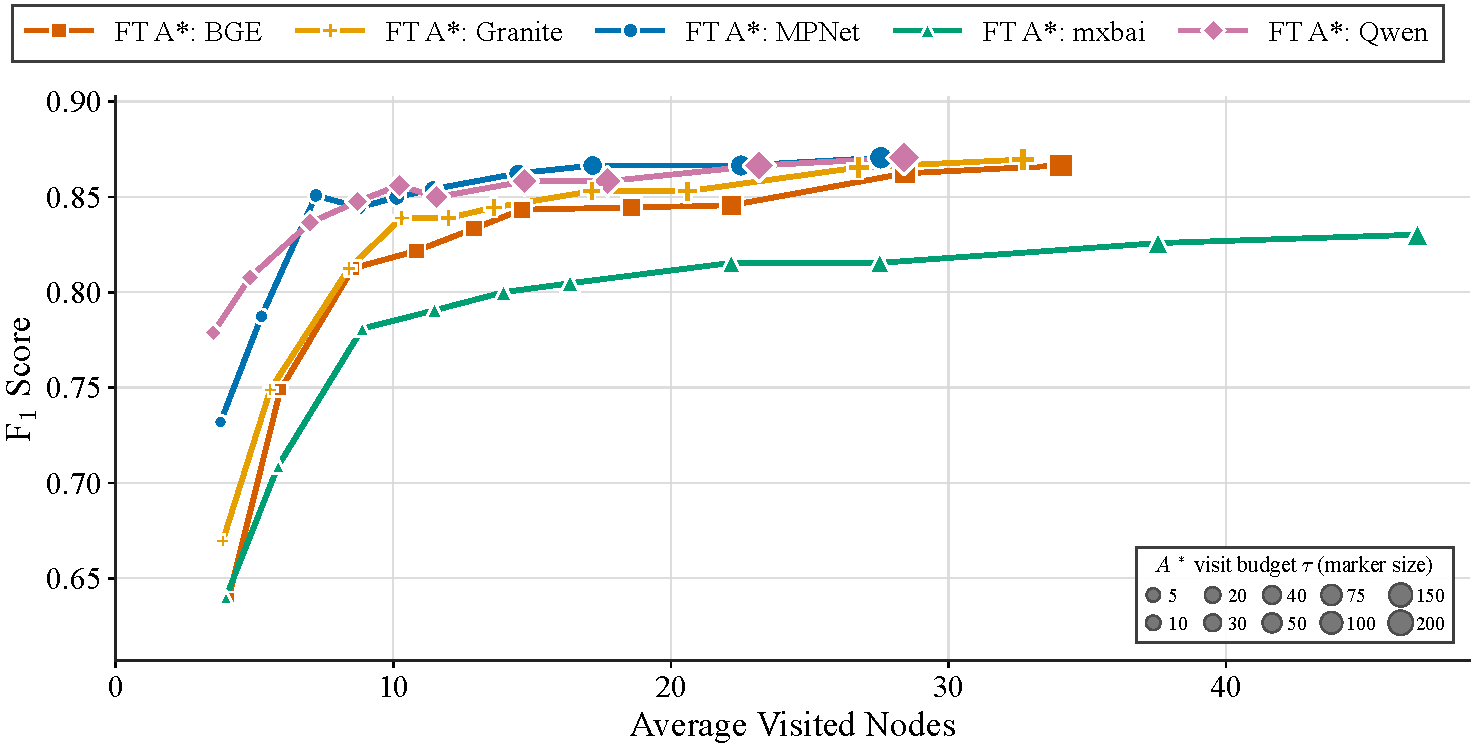
\includegraphics[width=\textwidth]{figures/budget_tradeoff_visited_nodes_linear.pdf}
    \caption{Efficiency--effectiveness trade-off for the five full-dimensional fine-tuned embedding models on MS MARCO validation with CauseNet Precision. F\textsubscript{1} score is shown against the measured average number of visited nodes, with marker size indicating the corresponding $A^*$ visit budget $\tau$.}
    \label{fig:budget-tradeoff}
\end{figure}

\section{Effect of Matryoshka Dimensionality}
\label{sec:results-matryoshka}

RQ2 examines the trade-off between effectiveness and efficiency across Matryoshka embedding dimensions. Figure~\ref{fig:metrics_summary} reports only capped fine-tuned models, using the same $p_{95}$-budget procedure across dimensions. Lower dimensions often reduce the visit budget, search effort, and runtime, although the effect is model-dependent and non-monotonic. For Granite, reducing the full 768-dimensional embedding to 32 dimensions lowers $\tau$ from 32 to 16, visited nodes from 11.0 to 7.1, and runtime from 1.9 to 1.2\,ms, while F\textsubscript{1} changes only slightly from \(82.3\%\) to \(81.9\%\). At 64 dimensions, F\textsubscript{1} instead improves to \(83.5\%\), with $\tau=23$, 9.1 visited nodes, and a runtime of 1.5\,ms. MPNet shows a similar intermediate optimum. At 64 dimensions, it retains the full model's \(82.4\%\) F\textsubscript{1} while reducing $\tau$ from 22 to 14, visited nodes from 7.5 to 6.1, and runtime from 1.7 to 1.3\,ms. Its two- and four-dimensional prefixes achieve higher F\textsubscript{1} scores of \(86.5\%\) and \(84.8\%\), but require 223.8 and 45.8 visited nodes, showing that lower dimensionality does not necessarily yield more efficient search. This instability at very low dimensions also appears for BGE and mxbai. Their two-dimensional variants reach \(83.6\%\) and \(79.2\%\) F\textsubscript{1}, respectively, but require 164.2 and 78.2 visited nodes. Qwen lies at the efficiency-oriented end of the trade-off, requiring only 3.8 visited nodes and 0.7\,ms at 768 dimensions, but reaching \(79.4\%\) F\textsubscript{1}. Different prefixes alter the embedding distances and therefore the order in which $A^*$ explores nodes. This helps explain why reducing dimensionality does not consistently reduce search effort. Overall, intermediate dimensions can provide better operating points than either the full embedding or very short prefixes while retaining sufficient information for effective search.

Among these operating points, MPNet-64 is the closest efficiency-oriented alternative to Granite-64, saving 2.9 node visits and 0.24\,ms while losing 1.1 percentage points of F\textsubscript{1}. On the global frontier, Granite-64 consequently obtains the higher Pareto-knee score, 0.285 compared with 0.257 for MPNet-64. Under the balanced effectiveness--efficiency objective, this effectiveness gain outweighs the modest additional search cost. MPNet-64, or Qwen-768 under a stricter latency constraint, could nevertheless be preferable when efficiency is prioritized more strongly. For the stated objective, the fine-tuned Granite-64 configuration with $\tau=23$ provides the best overall operating point and is therefore selected for the final test evaluation.

\begin{figure}[H]
    \centering
    \makebox[\textwidth][c]{%
        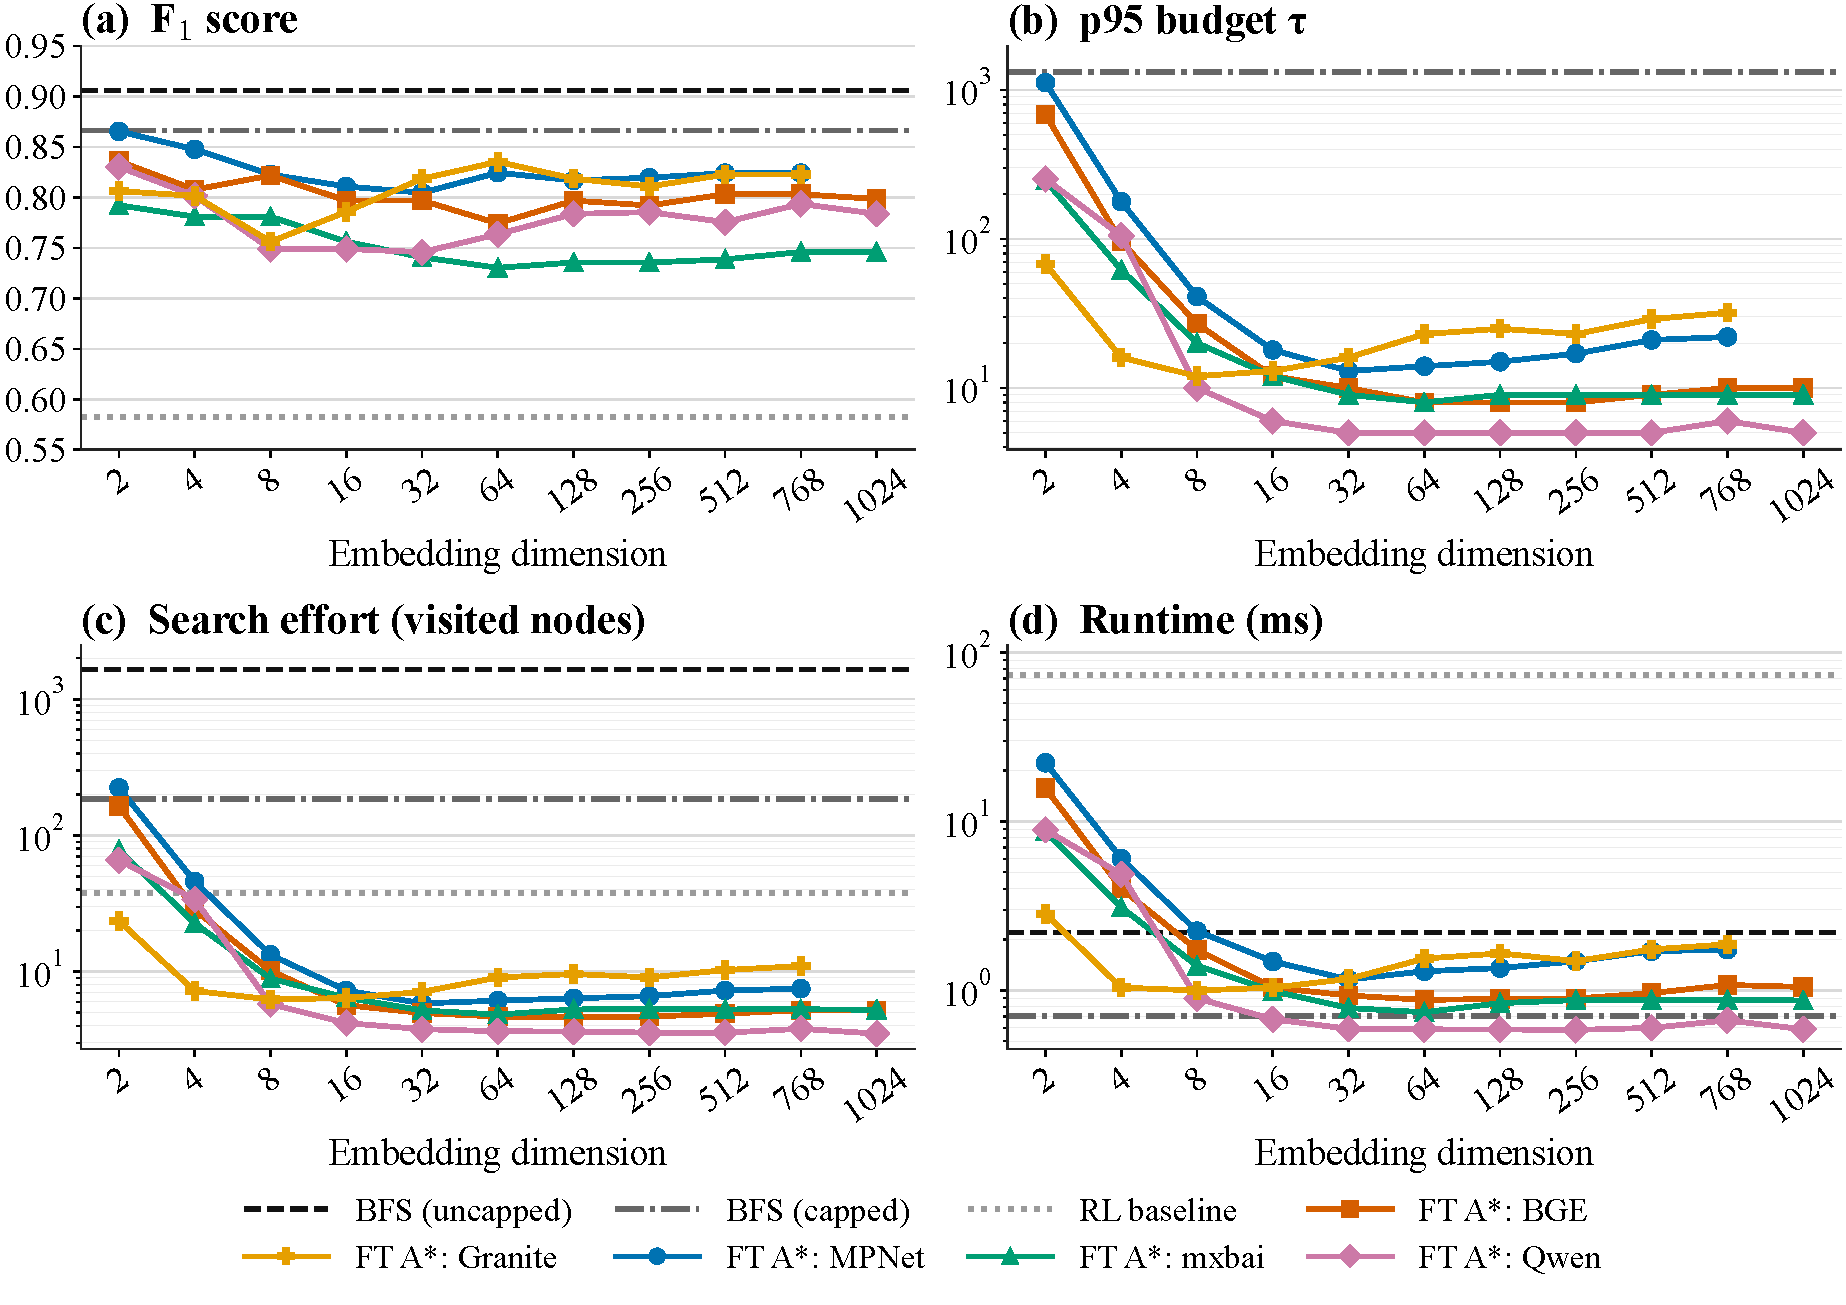
\includegraphics[width=1.05\textwidth]{figures/causenet_msmarco_valid_thesis_main.pdf}%
    }
        \caption{Validation performance of capped fine-tuned models on MS MARCO with CauseNet Precision across Matryoshka embedding dimensions. Shown are F\textsubscript{1}, the $p_{95}$ visit budget $\tau$, average visited nodes, and runtime. The budget, visited nodes, and runtime use logarithmic vertical axes.}
    \label{fig:metrics_summary}
\end{figure}

\section{Final Test Results}
\label{sec:results-comparison}

RQ3 compares the selected $A^*$ configuration with the BFS and RL baselines, while RQ4 examines its generalization across datasets and causal graph variants. Table~\ref{tab:final-results} reports the results on MS MARCO and SemEval for \mbox{CauseNet Precision}, CauseNet Full, and CEG Filtered. $A^*$ achieves a higher F\textsubscript{1} score, visits fewer nodes, and has a lower runtime than RL in all six settings. The comparison with BFS instead reveals an effectiveness--efficiency trade-off. On the smaller CauseNet Precision graph, BFS achieves the highest F\textsubscript{1} score on both datasets, whereas $A^*$ visits only 6.5 nodes on MS MARCO and 11.4 on SemEval. Capped BFS is faster in these settings, but visits 20.6 and 38.3 times as many nodes, respectively. This suggests that on smaller graphs, the overhead of embedding guidance can outweigh its savings in graph exploration.

On the larger CauseNet Full and denser CEG Filtered, the benefits of guided search become more pronounced. On CauseNet Full, $A^*$ visits only 7.5 nodes on MS MARCO and 14.2 on SemEval, compared with 30,099.3 and 160,715.3 for uncapped BFS. On MS MARCO, this substantial reduction in search effort comes with a lower F\textsubscript{1} score than either BFS variant. On SemEval, however, $A^*$ exceeds uncapped BFS by 9.5 percentage points and trails capped BFS by only 0.6 points. On CEG Filtered, $A^*$ attains an F\textsubscript{1} score of \(92.0\%\) on MS MARCO, matching capped BFS and slightly exceeding uncapped BFS while visiting only 2.3 nodes on average. Its F\textsubscript{1} score of \(68.5\%\) on SemEval lies between those of the two BFS variants, again with substantially fewer visited nodes and a lower runtime. These results demonstrate generalization beyond the CauseNet Precision--MS MARCO validation setting, with embedding guidance becoming more beneficial as graph exploration grows more expensive.

Tables~\ref{tab:f1-significance-causenet-precision}--\ref{tab:f1-significance-ceg} report paired stratified bootstrap tests for F\textsubscript{1} score differences between $A^*$ and each baseline. Positive $\Delta$ favors $A^*$ and negative $\Delta$ the baseline, with differences in percentage points. The 95\% confidence intervals are unadjusted, while $p_{\mathrm{Bonf.}}$ denotes the Bonferroni-adjusted $p$-value. The tests show that effectiveness depends on the graph and dataset. On MS MARCO, $A^*$ performs significantly worse than both BFS variants on \mbox{CauseNet Precision} and CauseNet Full, whereas neither comparison is significant on CEG Filtered. On SemEval, the pattern changes. $A^*$ significantly outperforms uncapped BFS on CauseNet Full, while its differences from both BFS variants on CauseNet Precision and capped BFS on CauseNet Full are not significant. The advantage over RL is more consistent, reaching significance on both datasets for both CauseNet variants, but not on CEG Filtered. Overall, the efficiency gains of $A^*$ do not imply a uniform loss in effectiveness. This is most apparent on CauseNet Full, where $A^*$ reduces graph exploration by several orders of magnitude while remaining competitive with BFS and outperforming RL.

\begin{table}[H]
\centering
\small
\setlength{\tabcolsep}{5pt}
\caption{Paired stratified bootstrap significance tests on CauseNet Precision.}
\label{tab:f1-significance-causenet-precision}
\begin{tabular}{@{}p{4.2cm}lrrrr@{}}
\toprule
\textbf{Dataset} & \textbf{Baseline} & $\boldsymbol{\Delta}$ & \textbf{95\% CI} & $\boldsymbol{p_{\mathrm{Bonf.}}}$ & \textbf{Sig.} \\
\midrule
MS MARCO & BFS (uncapped) & $-3.9$ & $[-6.7,-1.6]$ & $0.0123$ & yes \\
MS MARCO & BFS (capped)   & $-3.5$ & $[-6.2,-1.1]$ & $0.0306$ & yes \\
MS MARCO & RL             & $+16.4$ & $[+10.9,+22.5]$ & $0.0003$ & yes \\
SemEval  & BFS (uncapped) & $-5.2$ & $[-11.1,-0.2]$ & $0.1839$ & no \\
SemEval  & BFS (capped)   & $-4.9$ & $[-10.0,-0.8]$ & $0.1209$ & no \\
SemEval  & RL             & $+16.0$ & $[+7.0,+26.1]$ & $0.0048$ & yes \\
\bottomrule
\end{tabular}
\end{table}

\begin{table}[H]
\centering
\small
\setlength{\tabcolsep}{5pt}
\caption{Paired stratified bootstrap significance tests on CauseNet Full.}
\label{tab:f1-significance-causenet-full}
\begin{tabular}{@{}p{4cm}lrrrr@{}}
\toprule
\textbf{Dataset} & \textbf{Baseline} & $\boldsymbol{\Delta}$ & \textbf{95\% CI} & $\boldsymbol{p_{\mathrm{Bonf.}}}$ & \textbf{Sig.} \\
\midrule
MS MARCO & BFS (uncapped) & $-7.1$ & $[-10.6,-4.0]$ & $0.0006$ & yes \\
MS MARCO & BFS (capped)   & $-4.3$ & $[-7.2,-1.8]$ & $0.0084$ & yes \\
MS MARCO & RL             & $+13.0$ & $[+8.3,+17.9]$ & $0.0003$ & yes \\
SemEval  & BFS (uncapped) & $+9.5$ & $[+2.5,+15.6]$ & $0.0171$ & yes \\
SemEval  & BFS (capped)   & $-0.6$ & $[-6.9,+5.0]$ & $1.0000$ & no \\
SemEval  & RL             & $+24.8$ & $[+14.5,+35.5]$ & $0.0003$ & yes \\
\bottomrule
\end{tabular}
\end{table}

\begin{table}[H]
\centering
\small
\setlength{\tabcolsep}{5pt}
\caption{Paired stratified bootstrap significance tests on CEG Filtered.}
\label{tab:f1-significance-ceg}
\begin{tabular}{@{}p{4.2cm}lrrrr@{}}
\toprule
\textbf{Dataset} & \textbf{Baseline} & $\boldsymbol{\Delta}$ & \textbf{95\% CI} & $\boldsymbol{p_{\mathrm{Bonf.}}}$ & \textbf{Sig.} \\
\midrule
MS MARCO & BFS (uncapped) & $+1.0$ & $[+0.0,+3.2]$ & $1.0000$ & no \\
MS MARCO & BFS (capped)   & $+0.0$ & $[+0.0,+0.0]$ & $1.0000$ & no \\
MS MARCO & RL             & $+7.3$ & $[+0.6,+15.7]$ & $0.1671$ & no \\
SemEval  & BFS (uncapped) & $-0.2$ & $[-5.5,+4.5]$ & $1.0000$ & no \\
SemEval  & BFS (capped)   & $+0.2$ & $[-4.6,+4.6]$ & $1.0000$ & no \\
SemEval  & RL             & $+8.3$ & $[-2.2,+20.0]$ & $0.4260$ & no \\
\bottomrule
\end{tabular}
\end{table}

\begin{table}[t]
\centering
\small
\setlength{\tabcolsep}{2pt}
\sisetup{detect-weight=true}
\caption{Final test results for the selected fine-tuned Granite-64 $A^*$ configuration with $\tau=23$, compared with uncapped BFS (BFS-U), capped BFS (BFS-C), and the reinforcement learning baseline. CauseNet Prec. denotes CauseNet Precision. Precision (P), recall (R), and F\textsubscript{1} are reported in percent. T denotes runtime in milliseconds per query and N the average number of visited nodes. Asterisks mark F\textsubscript{1} scores that differ significantly from the selected $A^*$ configuration within each dataset--graph setting using a paired stratified bootstrap test with Bonferroni correction. Bold indicates the best value in each metric and dataset--graph setting, including ties.}
\label{tab:final-results}
\resizebox{\textwidth}{!}{%
\begin{tabular}{@{}llrrrrr@{\hspace{8pt}}rrrrr@{}}
\toprule
& & \multicolumn{5}{c}{\textbf{MS MARCO}} & \multicolumn{5}{c}{\textbf{SemEval}} \\
\cmidrule(lr){3-7}\cmidrule(lr){8-12}
\textbf{Graph} & \textbf{Approach}
& {\textbf{P}} & {\textbf{R}} & {\textbf{F\textsubscript{1}}} & {\textbf{T}} & {\textbf{N}}
& {\textbf{P}} & {\textbf{R}} & {\textbf{F\textsubscript{1}}} & {\textbf{T}} & {\textbf{N}} \\
\midrule
CauseNet Prec. & BFS-U
& 87.1 & {\bfseries 94.4} & {\bfseries 90.6$^{*}$} & 1.4 & 1157.3
& 89.2 & {\bfseries 87.9} & {\bfseries 88.5} & 6.6 & 6332.2 \\
CauseNet Prec. & BFS-C
& 87.5 & 93.0 & 90.2$^{*}$ & {\bfseries 0.5} & 134.9
& 91.8 & 84.8 & 88.2 & {\bfseries 1.2} & 436.7 \\
CauseNet Prec. & RL
& {\bfseries 89.2} & 58.0 & 70.3$^{*}$ & 67.7 & 32.0
& {\bfseries 97.1} & 51.5 & 67.3$^{*}$ & 114.4 & 38.3 \\
CauseNet Prec. & $A^*$
& 86.7 & 86.7 & 86.7 & 1.1 & {\bfseries 6.5}
& 92.6 & 75.8 & 83.3 & 1.8 & {\bfseries 11.4} \\
\midrule
CauseNet Full & BFS-U
& 85.6 & {\bfseries 94.7} & {\bfseries 89.9$^{*}$} & 59.5 & 30099.3
& 56.3 & {\bfseries 95.2} & 70.8$^{*}$ & 294.1 & 160715.3 \\
CauseNet Full & BFS-C
& 86.1 & 88.4 & 87.2$^{*}$ & 9.4 & 135.1
& 73.1 & 90.5 & {\bfseries 80.9} & 28.4 & 450.8 \\
CauseNet Full & RL
& {\bfseries 88.6} & 57.7 & 69.9$^{*}$ & 658.1 & 44.6
& {\bfseries 94.3} & 39.3 & 55.5$^{*}$ & 885.1 & 52.7 \\
CauseNet Full & $A^*$
& 86.7 & 79.4 & 82.9 & {\bfseries 7.2} & {\bfseries 7.5}
& 86.3 & 75.0 & 80.3 & {\bfseries 15.6} & {\bfseries 14.2} \\
\midrule
CEG Filtered & BFS-U
& 85.1 & {\bfseries 97.6} & 90.9 & 44.3 & 492.1
& 52.8 & {\bfseries 98.2} & {\bfseries 68.7} & 45.5 & 776.2 \\
CEG Filtered & BFS-C
& 87.0 & {\bfseries 97.6} & {\bfseries 92.0} & 5.8 & 30.2
& 52.9 & 96.5 & 68.3 & 9.1 & 42.4 \\
CEG Filtered & RL
& {\bfseries 89.2} & 80.5 & 84.6 & 5129.0 & 24.3
& {\bfseries 77.8} & 49.1 & 60.2 & 5131.9 & 54.7 \\
CEG Filtered & $A^*$
& 87.0 & {\bfseries 97.6} & {\bfseries 92.0} & {\bfseries 0.8} & {\bfseries 2.3}
& 56.2 & 87.7 & 68.5 & {\bfseries 4.4} & {\bfseries 7.2} \\
\bottomrule
\end{tabular}%
}
\end{table}


\section{Activation and Distance Ablation}
\label{sec:results-ablation}

This section analyzes the effects of the activation function and distance metric during fine-tuning. The same Granite model is trained with all four combinations of the ReLU or GELU activation function and Euclidean or cosine distance, while keeping all other settings fixed. The ablation is evaluated on CauseNet Precision, CauseNet Full, and CEG Filtered with both test datasets, using the selected 64-dimensional Matryoshka prefix and \(A^*\) budget \(\tau=23\).

Table~\ref{tab:activation-distance-ablation} reports the complete ablation results, while Figure~\ref{fig:ablation-tradeoff} summarizes the relationship between F\textsubscript{1} and search effort. ReLU--Euclidean provides the strongest overall trade-off across the evaluated settings. On both CauseNet variants, it achieves the highest F\textsubscript{1} and the lowest number of visited nodes. The results on CEG Filtered are more mixed. With \mbox{MS MARCO}, ReLU--Euclidean achieves the lowest search effort while tying for the highest F\textsubscript{1}. With SemEval, GELU--Cosine achieves the highest F\textsubscript{1}, whereas ReLU--Euclidean requires the fewest visited nodes. These results indicate that the preferred activation and distance combination can vary across graphs and datasets, although \mbox{ReLU--Euclidean} is the most consistent across settings.

Small runtime differences from Table~\ref{tab:final-results} result from separate evaluation runs. Among the ablation configurations, GELU is fastest in four of the six settings, including both CauseNet Full evaluations, but these gains generally coincide with lower F\textsubscript{1} and more visited nodes. For example, \mbox{GELU--Cosine} reduces runtime from \(14.9\) to \(7.4\)\,ms on CauseNet Full with SemEval compared with ReLU--Euclidean, but loses \(4.3\) F\textsubscript{1} points and visits \(1.2\) more nodes. Overall, ReLU--Euclidean provides the most consistent effectiveness--efficiency trade-off despite the runtime advantages of GELU in some settings.

\begin{figure}[H]
    \centering
    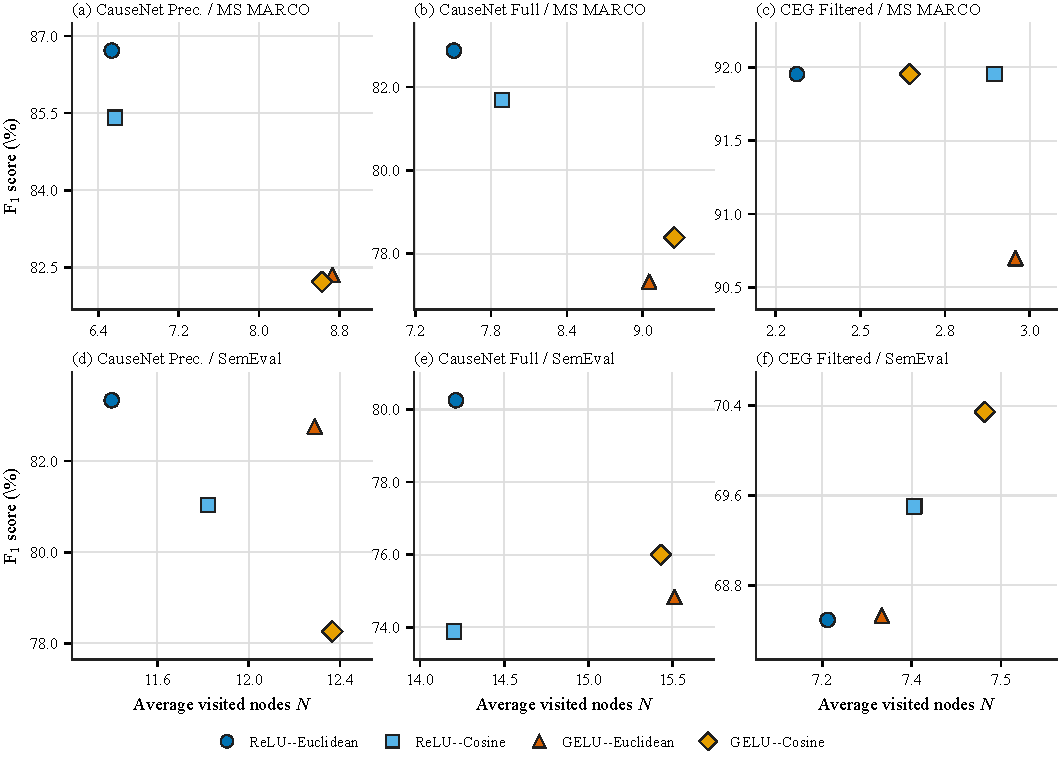
\includegraphics[width=\textwidth]{figures/ablation_tradeoff.pdf}
    \caption{Effectiveness--efficiency trade-off across activation and distance configurations. F\textsubscript{1} is plotted against average visited nodes across all six test settings.}
    \label{fig:ablation-tradeoff}
\end{figure}

\begin{table}[H]
\centering
\small
\setlength{\tabcolsep}{2pt}
\sisetup{detect-weight=true}
\caption{Activation and distance ablation for Granite-64 across all test settings with $\tau=23$. Bold indicates the best value per metric and setting, including ties.}
\label{tab:activation-distance-ablation}
\resizebox{\textwidth}{!}{%
\begin{tabular}{@{}ll
S[table-format=2.1]
S[table-format=2.1]
S[table-format=2.1]
S[table-format=2.1]
S[table-format=2.1]
@{\hspace{6pt}}
S[table-format=2.1]
S[table-format=2.1]
S[table-format=2.1]
S[table-format=2.1]
S[table-format=2.1]@{}}
\toprule
& & \multicolumn{5}{c}{\textbf{MS MARCO}}
& \multicolumn{5}{c}{\textbf{SemEval}} \\
\cmidrule(lr){3-7}\cmidrule(lr){8-12}
\textbf{Graph} & \textbf{Configuration}
& {\textbf{P}} & {\textbf{R}} & {\textbf{F\textsubscript{1}}} & {\textbf{T}} & {\textbf{N}}
& {\textbf{P}} & {\textbf{R}} & {\textbf{F\textsubscript{1}}} & {\textbf{T}} & {\textbf{N}} \\
\midrule
CauseNet Prec. & ReLU--Euclidean
& 86.7 & {\bfseries 86.7} & {\bfseries 86.7} & {\bfseries 1.0} & {\bfseries 6.5}
& 92.6 & {\bfseries 75.8} & {\bfseries 83.3} & 1.8 & {\bfseries 11.4} \\

CauseNet Prec. & ReLU--Cosine
& 87.0 & 83.9 & 85.4 & 1.1 & 6.6
& 94.0 & 71.2 & 81.0 & 1.9 & 11.8 \\

CauseNet Prec. & GELU--Euclidean
& 86.8 & 78.3 & 82.4 & 1.3 & 8.7
& {\bfseries 96.0} & 72.7 & 82.8 & {\bfseries 1.4} & 12.3 \\

CauseNet Prec. & GELU--Cosine
& {\bfseries 87.4} & 77.6 & 82.2 & 1.3 & 8.6
& 91.8 & 68.2 & 78.3 & 1.5 & 12.4 \\
\midrule

CauseNet Full & ReLU--Euclidean
& 86.7 & {\bfseries 79.4} & {\bfseries 82.9} & 6.9 & {\bfseries 7.5}
& 86.3 & {\bfseries 75.0} & {\bfseries 80.3} & 14.9 & {\bfseries 14.2} \\

CauseNet Full & ReLU--Cosine
& {\bfseries 87.3} & 76.7 & 81.7 & 6.5 & 7.9
& 79.5 & 69.0 & 73.9 & 12.3 & {\bfseries 14.2} \\

CauseNet Full & GELU--Euclidean
& 85.8 & 70.4 & 77.3 & 5.9 & 9.1
& {\bfseries 87.3} & 65.5 & 74.8 & 7.6 & 15.5 \\

CauseNet Full & GELU--Cosine
& 86.1 & 72.0 & 78.4 & {\bfseries 4.8} & 9.3
& 86.4 & 67.9 & 76.0 & {\bfseries 7.4} & 15.4 \\
\midrule

CEG Filtered & ReLU--Euclidean
& {\bfseries 87.0} & {\bfseries 97.6} & {\bfseries 92.0} & {\bfseries 0.8} & {\bfseries 2.3}
& 56.2 & 87.7 & 68.5 & 4.4 & {\bfseries 7.2} \\

CEG Filtered & ReLU--Cosine
& {\bfseries 87.0} & {\bfseries 97.6} & {\bfseries 92.0} & 1.4 & 2.9
& {\bfseries 58.3} & 86.0 & 69.5 & 4.4 & 7.4 \\

CEG Filtered & GELU--Euclidean
& 86.7 & 95.1 & 90.7 & 1.5 & 3.0
& 57.0 & 86.0 & 68.5 & {\bfseries 4.0} & 7.3 \\

CEG Filtered & GELU--Cosine
& {\bfseries 87.0} & {\bfseries 97.6} & {\bfseries 92.0} & 1.4 & 2.6
& 58.0 & {\bfseries 89.5} & {\bfseries 70.3} & 5.1 & 7.5 \\
\bottomrule
\end{tabular}%
}
\end{table}


\chapter{Discussion}
\label{chap:discussion}

The main advantage of embedding-guided $A^*$ lies in its ability to reduce search effort. It avoids the exhaustive exploration of BFS by prioritizing promising nodes and avoids the repeated neural inference of RL by relying on precomputed node embeddings. This makes the approach particularly suitable for large or dense causal graphs, where exhaustive traversal becomes increasingly expensive. This efficiency, however, comes with a trade-off because bounded exploration may terminate before an existing path is discovered, reducing recall. The reliability of the answers also depends on the underlying causal knowledge graph. Automatically constructed resources such as CauseNet and CEG may contain missing, noisy, ambiguous, or overly general relations, so a discovered path represents a connection encoded in the graph rather than definitive evidence of a real-world causal relationship. In addition, the approach assumes that causal relations can be meaningfully composed along a directed path, although causality is not necessarily transitive. Finally, the method is limited to binary causal questions. It determines whether a directed path between the graph nodes corresponding to the cause and effect can be found, but does not assess the quality, plausibility, or strength of the discovered causal relation. It also does not estimate causal effect sizes, compare alternative causes, or support interventional and counterfactual reasoning. These limitations restrict the proposed approach to efficient causal path discovery rather than general causal inference.



\chapter{Conclusion}
\label{chap:conclusion}

This thesis investigated whether a learned embedding-based heuristic can make $A^*$ a practical approach for binary causal question answering over large causal knowledge graphs. Questions of the form ``Does $A$ cause $B$?'' were modeled as directed reachability problems, with fine-tuned embedding distances guiding graph traversal. The final configuration uses Granite Embedding R2 with a 32-dimensional Matryoshka prefix, ReLU activation, Euclidean distance, and a search budget of $\tau=27$. The results show that embedding-guided $A^*$ substantially reduces traversal cost while maintaining competitive predictive performance. Its efficiency advantage is particularly pronounced on large or dense graphs such as CauseNet Full and CEG Filtered. On these graphs, $A^*$ is at least $9.8\times$ faster than capped BFS and $32.1\times$ faster than uncapped BFS, while visiting hundreds to thousands of times fewer nodes. It also outperforms the evaluated RL baseline in F\textsubscript{1} and runtime across all six final test settings. Overall, the findings demonstrate that learned embedding guidance provides an efficient alternative to exhaustive and policy-based traversal for binary causal graph search. Future work could address the limitations identified in this thesis. Adaptive, query-dependent search budgets could reduce recall loss caused by bounded exploration. Incorporating edge confidence, provenance, and path-quality estimation could improve robustness to noisy or ambiguous graph relations. Further work could also investigate the contextual validity of composed causal paths and extend the approach beyond binary reachability to tasks involving causal relation quality, effect strength, alternative causes, and interventional or counterfactual reasoning.

\bibliographystyle{unsrtnat}
\bibliography{literature}

\clearpage
\section*{Use of AI Tools}

OpenAI ChatGPT was used for language editing, formulation suggestions, consistency checks, and assistance with software development. All generated suggestions were reviewed, while responsibility for the scientific content, results, and cited sources remained entirely with the author.

\appendix
\chapter{Algorithmic Details}
\label{app:algorithmic-details}

This appendix provides implementation-level details of the two variants of embedding-guided $A^*$ search and the construction of search-aligned supervision. Algorithm~\ref{alg:bounded-astar-reachability} is the reachability-only variant used for binary evaluation. Because only a binary answer is required, it does not retain path information and returns as soon as the target is encountered among the successors of an expanded node. Algorithm~\ref{alg:bounded-astar-path} retains path information and is used when the discovered path itself is required, including supervision construction and interactive visualization. Algorithm~\ref{alg:training-dataset} uses this path-returning variant without a visit budget to construct $\mathcal{D}_s^d$ for the training and validation splits. Further details and source code are provided in the accompanying repository.\footnote{\url{https://git.webis.de/code-teaching/theses/thesis-kiafard.git}}

\begin{algorithm}[H]
\caption{Bounded embedding-guided $A^*$ reachability search}
\label{alg:bounded-astar-reachability}
\begin{algorithmic}[1]
\Require Directed graph $G=(V,E)$, source node $a$, target node $b$, embedding function $\phi$, distance function $d$, visit budget $\tau$
\Ensure \textsc{True} if a path from $a$ to $b$ is found, otherwise \textsc{False}
\If{$a=b$}
    \State \Return \textsc{True}
\EndIf
\State $open \gets$ priority queue containing $(0,0,a)$
\State $best\_g[a] \gets 0$
\State $closed \gets \emptyset$
\While{$open$ is not empty}
    \State $(f,g,u) \gets$ entry with smallest priority from $open$
    \If{$u=b$}
        \State \Return \textsc{True}
    \EndIf
    \If{$u \in closed$}
        \State \textbf{continue}
    \EndIf
    \State $closed \gets closed \cup \{u\}$
    \If{$\tau \neq -1$ \textbf{and} $|closed| > \tau$}
        \State \Return \textsc{False}
    \EndIf
    \If{$b \in N^{+}(u)$}
        \State \Return \textsc{True}
    \EndIf
    \ForAll{$v \in N^{+}(u)$ with $v \notin closed$}
        \State $g' \gets g + d(\phi(u),\phi(v))$
        \If{$v \notin best\_g$ \textbf{or} $g' < best\_g[v]$}
            \State $best\_g[v] \gets g'$
            \State $h' \gets d(\phi(v),\phi(b))$
            \State insert $(g'+h',g',v)$ into $open$
        \EndIf
    \EndFor
\EndWhile
\State \Return \textsc{False}
\end{algorithmic}
\end{algorithm}

\begin{algorithm}[H]
\caption{Bounded embedding-guided $A^*$ path search}
\label{alg:bounded-astar-path}
\begin{algorithmic}[1]
\Require Directed graph $G=(V,E)$, source node $a$, target node $b$, embedding function $\phi$, distance function $d$, visit budget $\tau$
\Ensure A path from $a$ to $b$ if found, otherwise $\emptyset$
\State $path\_links \gets [(a,\textsc{None})]$
\State $open \gets$ priority queue containing $(0,0,a,0)$
\State $best\_g[a] \gets 0$
\State $closed \gets \emptyset$
\While{$open$ is not empty}
    \State $(f,g,u,i) \gets$ entry with smallest priority from $open$
    \If{$u=b$}
        \State \Return path reconstructed from $path\_links$ at index $i$
    \EndIf
    \If{$u \in closed$}
        \State \textbf{continue}
    \EndIf
    \State $closed \gets closed \cup \{u\}$
    \If{$\tau \neq -1$ \textbf{and} $|closed| > \tau$}
        \State \Return $\emptyset$
    \EndIf
    \ForAll{$v \in N^{+}(u)$ with $v \notin closed$}
        \State $g' \gets g + d(\phi(u),\phi(v))$
        \If{$v \notin best\_g$ \textbf{or} $g' < best\_g[v]$}
            \State $best\_g[v] \gets g'$
            \State append $(v,i)$ to $path\_links$
            \State $j \gets |path\_links|-1$
            \State $h' \gets d(\phi(v),\phi(b))$
            \State insert $(g'+h',g',v,j)$ into $open$
        \EndIf
    \EndFor
\EndWhile
\State \Return $\emptyset$
\end{algorithmic}
\end{algorithm}

\begin{algorithm}[H]
\caption{Construction of search-aligned supervision}
\label{alg:training-dataset}
\begin{algorithmic}[1]
\Require Causal pairs $Q_s$ for split $s\in\{\mathrm{train},\mathrm{val}\}$, causal graph $G=(V,E)$, base embedding model $M$, distance function $d\in\{\mathrm{Cos},\mathrm{Euc}\}$
\Ensure Supervision dataset $\mathcal{D}_s^d$ of quadruples $(c,e,p,n)$
\State Precompute $\mathbf{z}_v \gets M(v)$ for all $v\in V$
\State Define $\phi(v) \gets \mathbf{z}_v$
\State $\mathcal{D}_s^d \gets \emptyset$
\State $cache \gets \emptyset$
\ForAll{$(A,B) \in Q_s$}
    \State Let $a,b\in V$ be the graph nodes corresponding to $A,B$
    \If{$(a,b) \in cache$}
        \State $P \gets cache[(a,b)]$
    \Else
        \State $P \gets$ path from unbounded $A^*$ on $G$ from $a$ to $b$ using $\phi$ and $d$
        \State $cache[(a,b)] \gets P$
    \EndIf
    \If{$|P| < 2$}
        \State \textbf{continue}
    \EndIf
    \For{$i \gets 0$ to $|P|-2$}
        \State $c \gets P_i$
        \State $p \gets P_{i+1}$
        \State $e \gets b$
        \ForAll{$n \in N^+(c) \setminus \{p\}$}
            \State $\mathcal{D}_s^d \gets \mathcal{D}_s^d \cup \{(c,e,p,n)\}$
        \EndFor
    \EndFor
\EndFor
\State \Return $\mathcal{D}_s^d$
\end{algorithmic}
\end{algorithm}

\end{document}
